\documentclass{beamer}
\mode<presentation> {

% The Beamer class comes with a number of default slide themes
% which change the colors and layouts of slides. Below this is a list
% of all the themes, uncomment each in turn to see what they look like.
\usepackage{graphicx}
\usepackage{svg}

\usepackage{graphicx}
\newcommand{\code}[1]{{\texttt{#1}}}
\usepackage{verbatim}
\usepackage{xspace}
%\usetheme{default}
%\usetheme{AnnArbor}
%\usetheme{Antibes}
%\usetheme{Bergen}
%\usetheme{Berkeley}
%\usetheme{Berlin}
%\usetheme{Boadilla}
%\usetheme{CambridgeUS}
%\usetheme{Copenhagen}
%\usetheme{Darmstadt}
%\usetheme{Dresden}
%\usetheme{Frankfurt}
%\usetheme{Goettingen}
%\usetheme{Hannover}
\usetheme{Ilmenau}
%\usetheme{JuanLesPins}
%\usetheme{Luebeck}
%\usetheme{Madrid}
%\usetheme{Malmoe}
%\usetheme{Marburg}
%\usetheme{Montpellier}
%\usetheme{PaloAlto}
%\usetheme{Pittsburgh}
%\usetheme{Rochester}
%\usetheme{Singapore}
%\usetheme{Szeged}
%\usetheme{Warsaw}

% As well as themes, the Beamer class has a number of color themes
% for any slide theme. Uncomment each of these in turn to see how it
% changes the colors of your current slide theme.
\usepackage{hyperref}

\usepackage{xcolor}
%\usecolortheme{albatross}
%\usecolortheme{beaver}
%\usecolortheme{beetle}
%\usecolortheme{crane}
%\usecolortheme{dolphin}
%\usecolortheme{dove}
%\usecolortheme{fly}
%\usecolortheme{lily}
%\usecolortheme{orchid}
%\usecolortheme{rose}
%\usecolortheme{seagull}
%\usecolortheme{seahorse}
%\usecolortheme{whale}
%\usecolortheme{wolverine}

%\setbeamertemplate{footline} % To remove the footer line in all slides uncomment this line
%\setbeamertemplate{footline}[page number] % To replace the footer line in all slides with a simple slide count uncomment this line

%\setbeamertemplate{navigation symbols}{} % To remove the navigation symbols from the bottom of all slides uncomment this line
}

\usepackage{graphicx} % Allows including images
\usepackage{booktabs} % Allows the use of \toprule, \midrule and \bottomrule in tables

%----------------------------------------------------------------------------------------
%	TITLE PAGE
%----------------------------------------------------------------------------------------

\title[Laboratoire d'ingénierie cognitive et sémantique (LinCS)]{MediatorBot: A Mediator bot for supporting collaborative E-learning using an Intelligent Tutor System} % The short title appears at the bottom of every slide, the full title is only on the title page

\author{Do Dung Vu \\ Supervisor: Prof. Sylvie Ratt\'e} % Your name

\institute[ETS] % Your institution as it will appear on the bottom of every slide, may be shorthand to save space
{
Département de génie logiciel et des TI \\ % Your institution for the title page
\medskip
\textit{do-dung.vu.1@ens.etsmtl.ca } % Your email address
}
\date{\today} % Date, can be changed to a custom date
\expandafter\def\expandafter\insertshorttitle\expandafter{%
	\insertshorttitle\hfill%
	\insertframenumber\,/\,\inserttotalframenumber}
\begin{document}

\begin{frame}
\titlepage % Print the title page as the first slide 
\end{frame}

\begin{frame}
\frametitle{Overview} % Table of contents slide, comment this block out to remove it
\tableofcontents % Throughout your presentation, if you choose to use \section{} and \subsection{} commands, these will automatically be printed on this slide as an overview of your presentation
\end{frame}

%----------------------------------------------------------------------------------------
%	PRESENTATION SLIDES
%----------------------------------------------------------------------------------------

%------------------------------------------------
\section{Introduction} % Sections can be created in order to organize your presentation into discrete blocks, all sections and subsections are automatically printed in the table of contents as an overview of the talk
%------------------------------------------------
\begin{frame}
\frametitle{Introduction}

\begin{center}
	

		\begin{figure}
			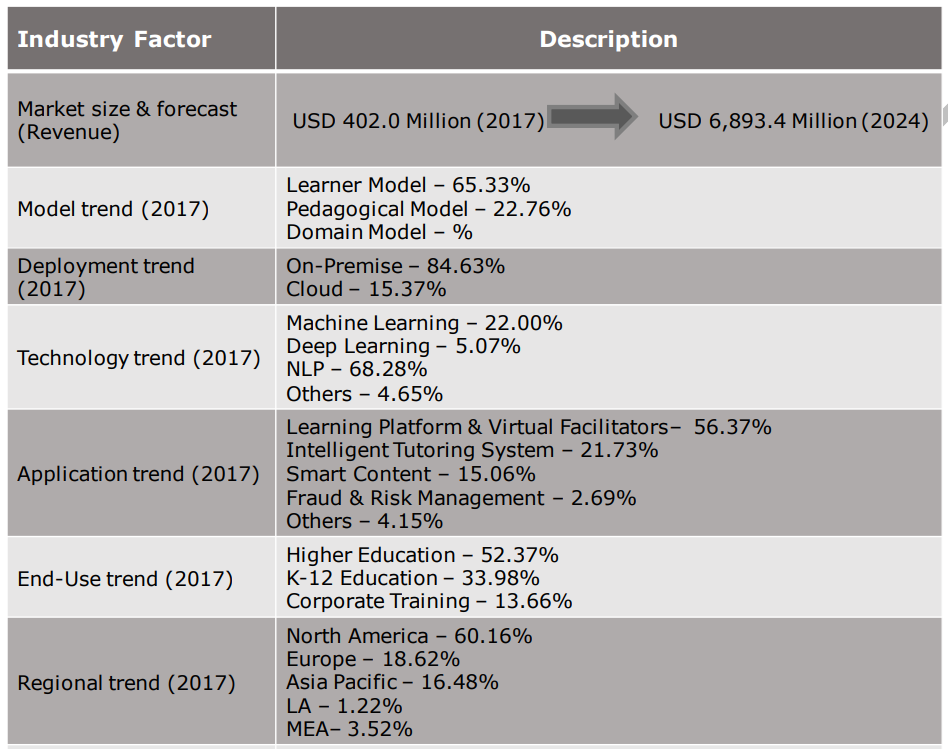
\includegraphics[width=65mm]{market2.png}
				
			
		\end{figure}
{\footnotesize 	AI in Education industry 3600 synopsis, 2013 – 2024}
	
{\tiny Source: AAAI, IEEE, WEF, IAAIL, Company Annual Reports, Hoovers, Primary Interviews, Global Market Insights}
\end{center}




\end{frame}

\begin{frame}
\frametitle{Introduction}
\begin{columns}
	\begin{column}{.45\textwidth}
		\begin{figure}
			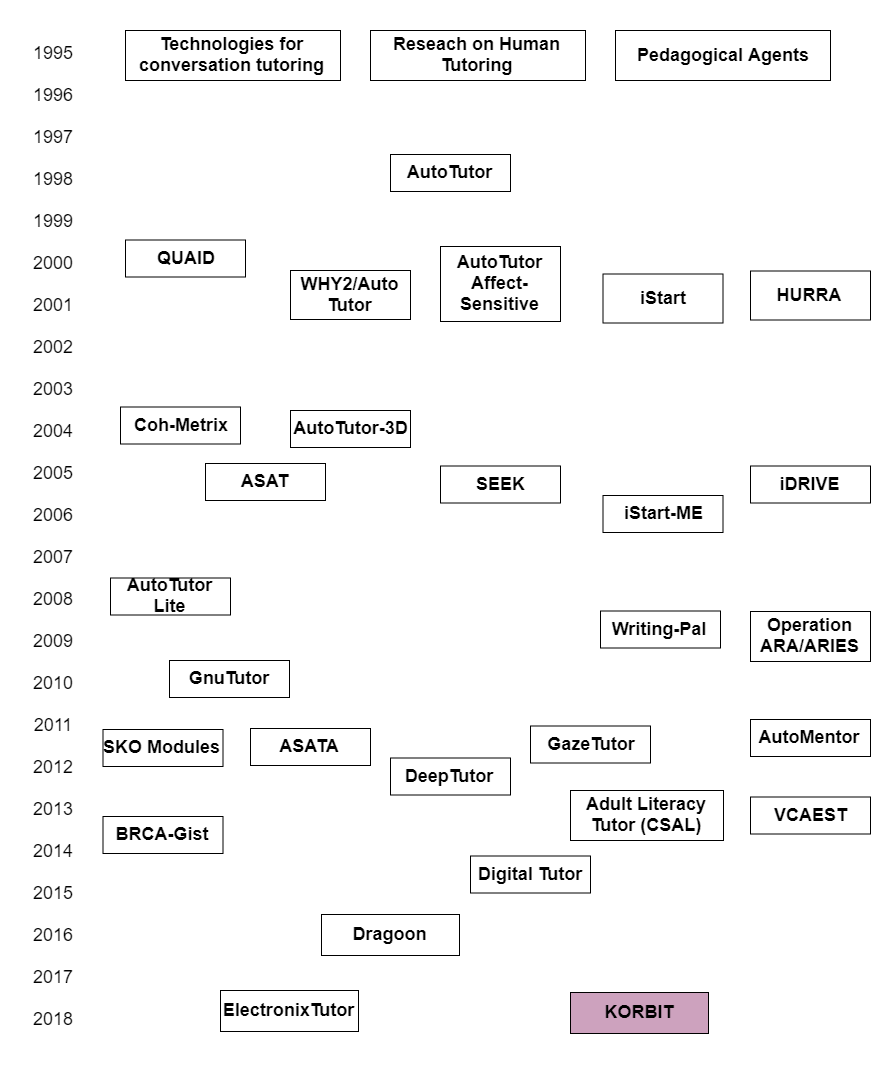
\includegraphics[width=45mm]{ht1s.png}
		\end{figure}
\begin{center}
	{\tiny 		\textbf{The time life of Intelligent Tutor System (ITS)}}
\end{center}
	\end{column}
	
	\begin{column}{.55\textwidth}
	\begin{block}{ITS main purposes: }
		\begin{itemize}
			\item Help students construct expressions of material as answers to questions and solutions to challenging problems
			\item Ask questions that tap deep levels of reasoning and that involve collaboration
			\item Solve problems that involve deep argumentation
		\end{itemize} 
	\end{block}
		

	\end{column}
\end{columns}
\end{frame}




\section{Problem statement} % Sections can be created in order to organize your presentation into discrete blocks, all sections and subsections are automatically printed in the table of contents as an overview of the talk
%------------------------------------------------

\begin{frame}
\frametitle{Context}
\begin{columns}
	\begin{column}{.5\textwidth}
		\begin{itemize}
			\item Online group learning on a given domain-specific (e.g., statistic)
			\item The group must discuss about a given topic or assignment (e.g., \url{https://mydalite.org/en/})
			\item The Intelligence Tutor System (ITS) help Professor to monitor the progress of students and Admin to encourage their study
		\end{itemize}
	\end{column}
	\begin{column}{.5\textwidth}
\begin{figure}
	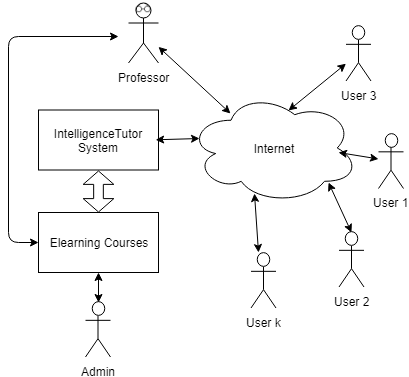
\includegraphics[width=45mm]{se1.png}
\end{figure}
\end{column}
\end{columns}

\end{frame}
\begin{frame}
\frametitle{Literature survey}
\begin{itemize}
	\item An ITS monitors  students' knowledge, skills, and psychological
	characteristics  and response \cite{Sottilare}
	\item Conversational agents have talking heads that
	speak, point, gesture, and exhibit facial expressions.
\cite{Johnson2016}
	
	\item AutoTutor and its progenies \cite{Graesser2016} help students learn by holding a conversation in natural language
	\item Agent intervention aiming to link students' contributions to previously acquired knowledge can improve both individual and group studying when implemented in the context of a collaborative learning activity in higher education \cite {Tegos}
\end{itemize}
\end{frame}
\begin{frame}
\frametitle{Reference}
\begin{thebibliography}{01}
{\scriptsize 	\bibitem{Sottilare}	[1] Sottilare, R, Graesser, AC, Hu, X, Goldberg, B (Eds.) (2014). Design recommendations
for intelligent tutoring systems: instructional management, (vol. 2). Orlando:
Army Research Laboratory
\bibitem{Johnson2016} [2] 	Johnson, WL, \& Lester, JC. (2016). Face-to-face interaction with pedagogical
agents, twenty years later. International Journal of Artificial Intelligence in
Education, 26(1), 25–36.
		
\bibitem{Graesser2016} [3]	Graesser, AC. (2016). Conversations with AutoTutor help students learn.
International Journal of Artificial Intelligence in Education, 26, 124–132	

 \bibitem{Tegos} [4] Tegos,  S.,  \&  Demetriadis,  S.  (2017). Conversational  Agents  Improve Peer  Learning  through  Building  on Prior  Knowledge.Educational Technology \& Society, 20(1), 99–111}
\end{thebibliography}
\end{frame}
\begin{frame}
\frametitle{Problem statement | Context}
The seven most commonly in Online Learning found in the literature are the following\footnote{{\tiny Jianxia Du, Chuang Wang, Mingming Zhou, Jianzhong Xu, Xitao Fan \& Saosan Lei (2018) Group trust, communication media, and interactivity: toward an integrated model of online collaborative learning, Interactive Learning Environments, 26:2, 273-286,}
}:
{\footnotesize \begin{itemize}
	\item (1): the student has conflicts works in the group
	\item (2): the selection of the groups is not good
	\item (3): the students don't have enough group-work skills
	\item (4):  some students want to work alone or become the free-riders
	\item (5):  the possible inequalities of student abilities appears in the group
	\item (6):  some members do not commit to working in the group with their responsibilities
	\item (7): the assessment of individuals within the groups is not fair
\end{itemize}}


%S. Tegos, \& S. Demetriadis, "Conversational Agents Improve Peer Learning through Building on Prior Knowledge", in Educational Technology \& Society, 20 (1), 99--111, 2017
\end{frame}

\begin{frame}
\frametitle{Problem statement|Context}
Most of these problems above of online group learning are inter-related

		\begin{figure}
			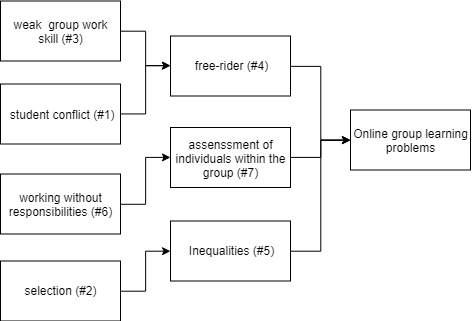
\includegraphics[width=45mm]{p21.png}
		\end{figure}






%S. Tegos, \& S. Demetriadis, "Conversational Agents Improve Peer Learning through Building on Prior Knowledge", in Educational Technology \& Society, 20 (1), 99--111, 2017
\end{frame}

\begin{frame}
\frametitle{Problem statement| Main problem}

\begin{columns}
	\begin{column}{.55\textwidth}
	\begin{figure}
		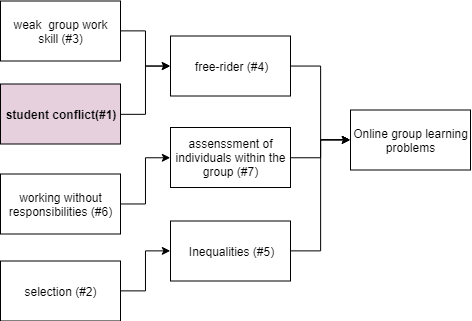
\includegraphics[width=45mm]{p22.png}
	\end{figure}
	\end{column}
\begin{column}{.55\textwidth}
	\#3: solved by orientation training from admin \\
	\#6, \#2: solved by professor\\
	\textcolor{blue}{\textbf{\#1: solved by ITS system}}
\end{column}
\end{columns}
\begin{flushleft}
	
\end{flushleft}

$\rightarrow$ in the ITS based on Dialogue System, there are other potential problems in the online group learning that have not been dealt with

$\rightarrow$	We want to solve the problem of conflict students with the teamwork. 








%S. Tegos, \& S. Demetriadis, "Conversational Agents Improve Peer Learning through Building on Prior Knowledge", in Educational Technology \& Society, 20 (1), 99--111, 2017
\end{frame}


\begin{frame}
\frametitle{Problem statement|Scenario}
\begin{columns}[onlytextwidth]
	\begin{column}{.45\textwidth}
		\begin{figure}
			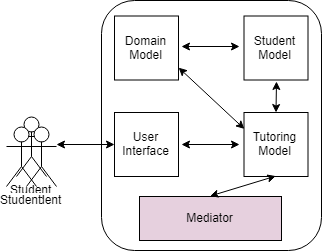
\includegraphics[width=.8\textwidth]{pp1}

				\caption{ITS with Mediator}
		\end{figure}
	\end{column}
	\hfill
	\begin{column}{.45\textwidth}
		\begin{figure}
			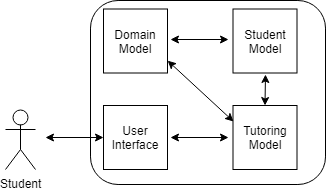
\includegraphics[width=.8\textwidth]{pp2}
					\caption{Original ITS [*]}

					
		\end{figure}
	
	\end{column}

\end{columns}
\begin{flushright}
	
\end{flushright}
{\tiny 					[*] N. T-Nghe and L. S-Thieme, "Multi-Relational Factorization Models for Student Modeling in Intelligent Tutoring Systems",  17th International Conference on Knowledge and Systems Engineering (KSE) 2015
}
\end{frame}
\begin{frame}
\frametitle{Problem statement| Scenario}
\begin{center}
	
\end{center}
\textcolor{blue}{\textbf{MediatorBot} generates the hints, identifies the debated problem, the opportunities for intervention, and answers the related topic question of students to encourage the users to collaborate more effectively in the online group learning with low price in the specific-domain}
\end{frame}
\begin{frame}


\frametitle{Problem statement| Scenario}


	   \begin{columns}[t]

		\column{.5\textwidth}
	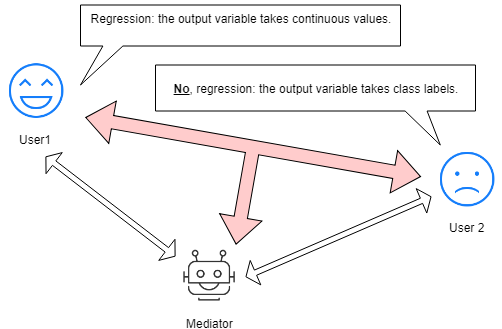
\includegraphics[width=.8\columnwidth]{p3}
 1
	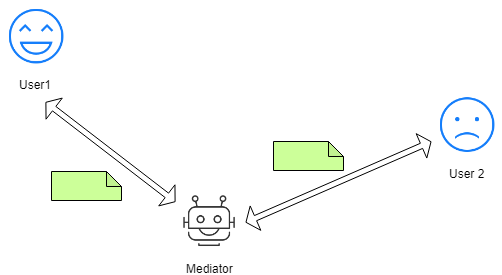
\includegraphics[width=.8\columnwidth]{p5}
3
	\column{.5\textwidth}
	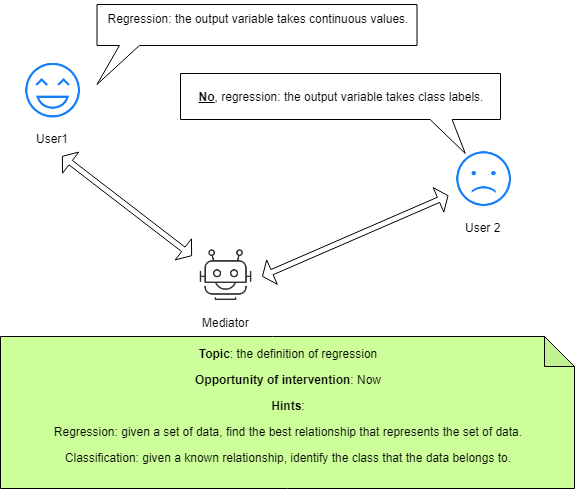
\includegraphics[width=.8\columnwidth]{p4}
2
	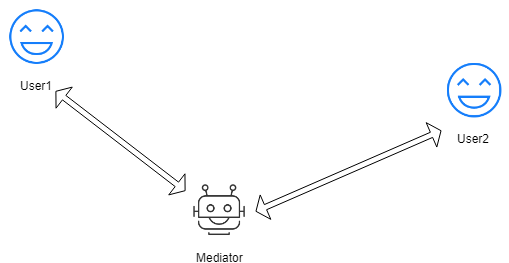
\includegraphics[width=.8\columnwidth]{p6}
4

\end{columns}


\end{frame}









%S. Tegos, \& S. Demetriadis, "Conversational Agents Improve Peer Learning through Building on Prior Knowledge", in Educational Technology \& Society, 20 (1), 99--111, 2017

\begin{comment}
\section{Literature Review} % Sections can be created in order to organize your presentation into discrete blocks, all sections and subsections are automatically printed in the table of contents as an overview of the talk
%------------------------------------------------
\begin{frame}
\frametitle{Literature Review}
 \begin{itemize}
{\footnotesize  \item  The important features and chatbot states to be considered in  conversational user
 interface  design  for  specific  domain (e.g., task, duty specification, predict, personalize) in [2]
 	\item A teacher-configurable agent intervention mode 
 	encourages peers to build on their prior knowledge, drawing on the academically productive talk (APT) 	discourse framework is presented in [3]
 	\item The use of conversational agents to scaffold online collaborative learning discussions through an
 	approach called academically productive talk (APT) is investigated in [4].
 	\item A socially capable conversational tutor that supports teams of three (or more) learners in a
 	design task even though there is still
 	room for improvement to match human performance [5]}
 \end{itemize}

\end{frame}
\begin{frame}
\frametitle{Reference}
{\scriptsize \par [1] S. Tegos, \& S. Demetriadis, "Conversational Agents Improve Peer Learning through Building on Prior Knowledge", in Educational Technology \& Society, 20 (1), 99--111, 2017.}
{\scriptsize \par [2] A. Fadhil, "Domain Specific Design Patterns: Designing For Conversational User Interfaces", https://arxiv.org/pdf/1802.09055.pdf}
{\scriptsize \par [3]  S. Tegos, \& S. Demetriadis, "Conversational Agents Improve Peer Learning through Building on Prior Knowledge", in Educational Technology \& Society, 20 (1), pp. 99--111, 2017. }
{\scriptsize \par [4] G. Dyke, D. Adamson, I. Howley and C. P. Rosé, "Enhancing Scientific Reasoning and Discussion with Conversational Agents," in IEEE Transactions on Learning Technologies, vol. 6, no. 3, pp. 240--247, 2013. }
{\scriptsize \par [5] R. Kumar ,H. Ai, J.L. Beuth , C.P. Rosé, "Socially Capable Conversational Tutors Can Be Effective in Collaborative Learning Situations", in: Aleven V., Kay J., Mostow J. (eds) Intelligent Tutoring Systems. ITS 2010.}

\end{frame}
\end{comment}

\section{Motivations} % Sections can be created in order to organize your presentation into discrete blocks, all sections and subsections are automatically printed in the table of contents as an overview of the talk
%------------------------------------------------
\begin{frame}
\frametitle{Motivations}
\begin{columns}
	\begin{column}{.55\textwidth}
		\begin{figure}
			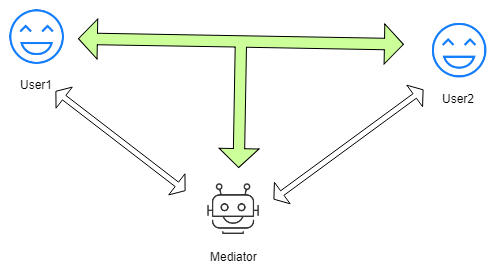
\includegraphics[width=55mm]{m1.png}
		\end{figure}

	\end{column}
	
	\begin{column}{.55\textwidth}
		\begin{itemize}
			\item Future state-of-the-art interventions with low price for intelligent tutor system
			\item Encourage student collaboration online
			\item Easily scalable 
		
			
		\end{itemize}
	\end{column}
\end{columns}
\end{frame}


\section{Objectives} % Sections can be created in order to organize your presentation into discrete blocks, all sections and subsections are automatically printed in the table of contents as an overview of the talk
%------------------------------------------------
\begin{frame}
\frametitle{Objectives}
{\large \textcolor{blue}{\textbf{Main objective:}}} Propose a smart Mediator to support constructive discussion based on the Intelligent Tutor System:

\begin{itemize}
	\item Generate hints to help users solve the topic or problem automatically
	\item    Identify the debated problem
	\item Intervene in the conversation to resolve the conflict
\end{itemize}

\end{frame}



\section{Methodology} % Sections can be created in order to organize your presentation into discrete blocks, all sections and subsections are automatically printed in the table of contents as an overview of the talk
%------------------------------------------------
\begin{frame}
\frametitle{Mediator system}
\begin{figure}
	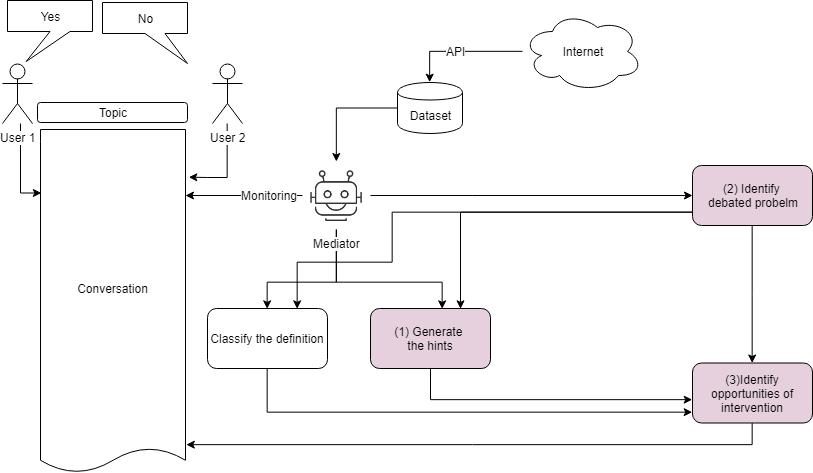
\includegraphics[width=80mm]{2.png}
\end{figure}

\end{frame}
\begin{frame}
\par 	\textbf{(1)  Generate hints to help users solve the topic or problem automatically}
\par \textcolor{gray}{(2) Identify the debated problem }
\par (3) \textcolor{gray}{ Intervene in the conversation to clarify the problem }
\end{frame}

\begin{frame}
\frametitle{Objective 1| Structure}

Generate hints to help users solve the topic or problem automatically



\begin{center}
			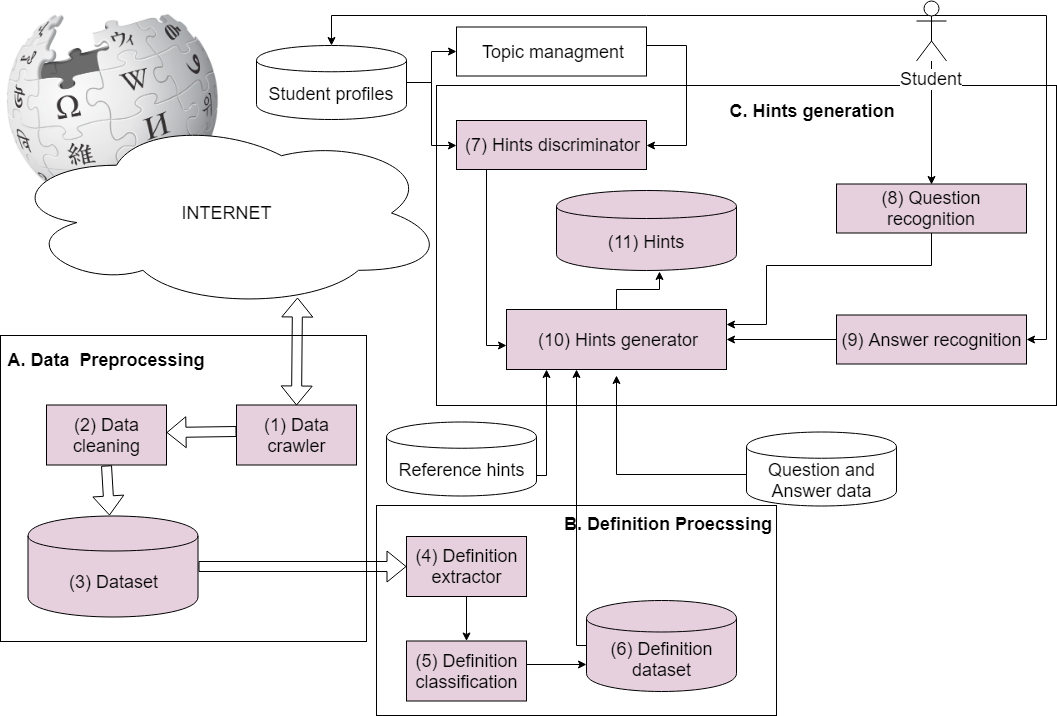
\includegraphics[width=70mm]{23.png}
\end{center}

\end{frame}
\begin{frame}

\frametitle{Objective 1 | Methodology | A. Data preprocessing}
\begin{columns}
\begin{column}{.5\textwidth}

(1) Data crawler: crawling data from wikipedia with a given domain-specific (e.g., statistic)\\

(2) Data cleaning: clean the unicode, convert xml equation to latex equation, clean punctuation, split raw text to line by line sentence\\
(3) Dataset: save data to the tsv file with it fields: title, link, content\\
\end{column}
\begin{column}{.5\textwidth}
		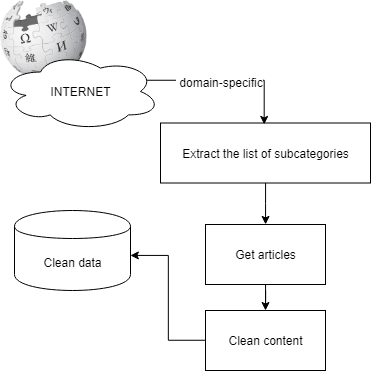
\includegraphics[width=50mm]{cr.png}
\end{column}

\end{columns}
\end{frame}
\begin{frame}
\frametitle{Objective 1 | Methodology | B. Definition processing}
(4) Definition extractor: Extract the description of each concept\\
(5) Definition classification: classify type of definition based on supervisor algorithm (Good/Not Good)\\
$\rightarrow$ Using the oversampling methodology to reweight the Good and Not Good samples
(6) Definition dataset: definition with its' label
\end{frame}
\begin{frame}
\frametitle{Objective 1 | Methodology | B. Definition processing | Definition extractor}
\begin{columns}
		\begin{column}{.5\textwidth}
		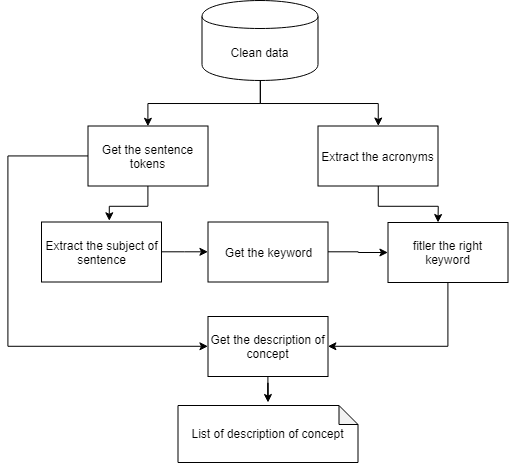
\includegraphics[width=50mm]{df1.png}
	\end{column}
	\begin{column}{.65\textwidth}
		
		\begin{itemize}
			\item Split raw text dataset to the sentence tokens
			\item Extract the technical keyword acronyms
			\item Extract subject (noun phase) $\leftarrow$ Get the keyword (concept)
			\item Filter the right keyword (concept)
			\item Get the description of concept
			\item Save the list (dict) description of conecept which is called dictionary of definition
		\end{itemize}
	\end{column}

	
\end{columns}
\end{frame}
\begin{frame}
\frametitle{Objective 1 | Methodology | B. Definition processing | Definition classification}
\begin{columns}

	\begin{column}{.55\textwidth}
		\begin{itemize}
			\item Extract the features $\leftarrow$ score table
			\item Save the score table to the definition dataset
			\item Classify the G/NG definition based on supervised learning algorithm
			\item Save the classification model
		\end{itemize}
	
	\end{column}
	\begin{column}{.55\textwidth}
	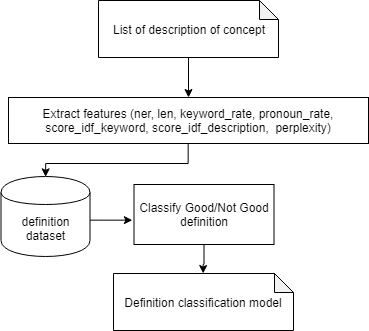
\includegraphics[width=50mm]{dc1.png}
\end{column}
	
	
\end{columns}
\end{frame}
\begin{frame}
\frametitle{Objective 1 | Methodology | B. Definition processing | Definition classification}
{\tiny \begin{table}[]
	\begin{tabular}{|l|l|lll}
		\cline{1-2}
		\textbf{Features}             & \textbf{Summary}              &  &  &  \\ \cline{1-2}
		\code{length\_of\_keyword}  & the number words in the keyword    &  &  &  \\ \cline{1-2}
		\code{length\_of\_description} & the number words in the description &  &  &  \\ \cline{1-2}
		\code{score\_keyword}          & inverse document frequency of keyword          & &  &  \\ \cline{1-2}
		\code{score\_description}          & inverse document frequency of concepts description          & &  &  \\ \cline{1-2}
		
		\code{ner\_in\_description}          & name of entity recognition within the description        & &  &  \\ \cline{1-2}
		
		
		\code{coreference\_in\_description}          & compute the coreference resolution score         & &  &  \\ \cline{1-2}
		
		\code{type\_of\_word}          & recognize type of word (verb, noun, etc.,)        & &  &  \\ \cline{1-2}
		
		\code{non\_of\_word}          & recognize the none of word (symbol, number, etc.,)        & &  &  \\ \cline{1-2}
		\code{pronouns\_rate}          &  the rate of $\frac{pronouns}{nouns}$  & &  &  \\ \cline{1-2}
		\code{keyword\_rate}          &  the rate of $\frac{keyword\_position}{length\_of\_description}$  & &  &  \\ \cline{1-2}
		\code{perplexity}          & the real value of perplexity of desciption  & &  &  \\\cline{1-2}
		\code{likelihood\_score}          & \begin{tabular}[c]{@{}l@{}}the log-likelihood probability score of description\\ based on sum of probability term by using language \\model based on RNN \end{tabular} & &  &  \\ \cline{1-2}
	\end{tabular}
	\caption{Features of definition}
\end{table}}
\end{frame}
\begin{frame}
\frametitle{Objective 1 | Methodology | B. Definition processing | Definition classification| Example}
{\tiny \begin{table}[]
		\begin{tabular}{|l|l|l|l|l|l|l|}
			\hline
			key & definitnion & label & \begin{tabular}[c]{@{}l@{}}score\\ keyword\end{tabular} & \begin{tabular}[c]{@{}l@{}}score\\ definition\end{tabular} & ... & \begin{tabular}[c]{@{}l@{}}likelihood\\ score \\ definitnion\end{tabular} \\ \hline
			\begin{tabular}[c]{@{}l@{}}Linear\\   regression\end{tabular}   & \begin{tabular}[c]{@{}l@{}}In statistics, linear   regression \\is a linear approach to \\ modelling the relationship between a \\scalar response (or dependent variable)\\  and one or more explanatory\\ variables  (or independent variables).\end{tabular}              & Positive      & 14.58                                                        & 130.53                                                                     & ...                & 10.64                                                                                     \\ \hline
		\begin{tabular}[c]{@{}l@{}}linear \\regression\\   models\end{tabular}	&  \begin{tabular}[c]{@{}l@{}}The numerical methods for  \\linear least squares are\\ important because linear regression\\ models are among   the\\ most important types of\\ model, both as formal statistical\\ models and   exploration of data-sets.\end{tabular}            &     Negative   &  20.78                                                                 &                                   146.77                                     &   ...  &                         10.49                                                               \\ \hline
		\end{tabular}
\end{table}}
\end{frame}
\begin{frame}
\frametitle{Objective 1 | Methodology | C. Hint generation}
(7) Hints discriminator: classify level of hints based on the student profiles \\
(8) Question recognition: recognize question of student\\
(9) Answer recognition: recognize answer of student \\

(10) Hints generator: generate hint based on hint types, level, and language model \\
\end{frame}


\begin{frame}
\frametitle{Objective 1 | Methodology | C. Hint generation | Hints discriminator }
\begin{columns}
	
	\begin{column}{.55\textwidth}
		\begin{itemize}
			\item Classify the students' level based on their profile
			\item Discriminate hints based on level of student
			
		\end{itemize}
		
	\end{column}
	\begin{column}{.55\textwidth}
		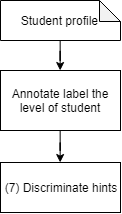
\includegraphics[width=25mm]{hd1.png}
	\end{column}
\end{columns}
\end{frame}
\begin{frame}
\frametitle{Objective 1 | Methodology | Hint generating | Question \& Answer recognition }
(8) Question recognition: Recognize the users' questions\\
(9) Answer recognition: Recognize the users' answers
\begin{center}
		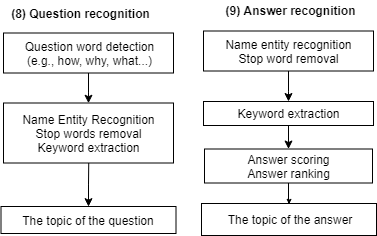
\includegraphics[width=65mm]{qa3.png}
\end{center}
\end{frame}
	

\begin{frame}
\frametitle{Objective 1 | Methodology | C. Hint generation| Hint generator}
	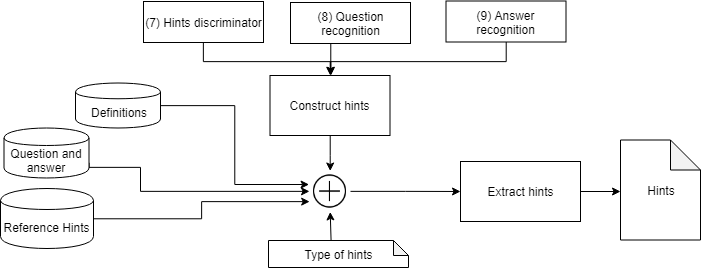
\includegraphics[width=90mm]{ht2.png}
\end{frame}
\begin{frame}
\frametitle{Objective 1 | Methodology | C. Hint generation| Hint generator| Construct hints}
* The hints are phrased in the form of "Think about X" or "Consider X" where X is the part of expectation answer. \\
* Using Linear regression model based on the features: 
{\tiny \begin{table}[]
	\begin{tabular}{|l|l|lll}
		\cline{1-2}
		\textbf{Features}             & \textbf{Summary}              &  &  &  \\ \cline{1-2}
		\code{length\_of\_hint}  & the number words in the hint     &  &  &  \\ \cline{1-2}
		\code{overlap\_question\_hint} & the rate of overlap between question and hint &  &  &  \\ \cline{1-2}
		\code{score\_keyterm}          & inverse document frequency of keyterm in hint          & &  &  \\ \cline{1-2}
		\code{keyhint\_keyquestion\_ratio}          & the ratio of $\frac{number\_of\_keyhint}{number\_of\_keyquestion}$     &  &  &  \\ \cline{1-2}
		\code{topic\_overlap}          & content overlap between the question and hint     &  &  &  \\ \cline{1-2}
		
		\code{pronouns\_rate}          &  the rate of $\frac{pronouns}{nouns}$ in hint  & &  &  \\ \cline{1-2}
		\code{keyword\_rate}          &  the rate of $\frac{keyword\_position}{length\_of\_hint}$  & &  &  \\ \cline{1-2}
		\code{perplexity}          & the real value of perplexity of hint  & &  &  \\ \cline{1-2}
		\code{ner\_in\_hint}          & name of entity recognition within the hint        & &  &  \\
		 \cline{1-2}
		 	\code{score\_of\_hint}          & \begin{tabular}[c]{@{}l@{}}the log-likelihood probability score of hints\\ based on sum of probability terms  by using language \\model based on RNN\end{tabular}       & &  &  \\
		 		 \cline{1-2}
	\end{tabular}
	\caption{Features of hints}
	\label{tab:3}
\end{table}}

\end{frame}
\begin{frame}
\frametitle{Objective 1 | Methodology | C. Hint generation| Hint generator| Construct hints| Example}


{\tiny \textbf{Question:\\}
\colorbox{green!30}{\begin{tabular}[c]{@{}l@{}}You are given a dataset of images of wildlife in Africa.\\ You are tasked with building a model which can identify animals in the images. \\
Is this a regression or classification problem? Explain why?\end{tabular}    }}\\
{\tiny \textbf{Hints:}}
{\tiny \begin{itemize}
	\item Recall that each animal is a class.
	\item Recall that each animal is a discrete class.
	\item Consider that each animal is a separate class.
	\item Consider that we are choosing between a set of categories.
	\item Think about the following: we are choosing between discrete-valued output variables.
	\item Consider that each image can contain several animals, and therefore the model must predict the existence of each type of animal.
	
\end{itemize}}
\end{frame}
\begin{comment}
\begin{frame}
\frametitle{Objective 1 $|$ (A) Pattern detection}
\par + Extract the subject or object  of each sentences in the conversation to get the candidate pattern\footnote{https://spacy.io/} based on syntax tree 
\par + Compute the tf-idf score of each pattern
	
\begin{equation}
W^{PT} = \prod_{k}{TFIDF(term_k)}
\end{equation}


\end{frame}
\begin{frame}
\frametitle{Objective 1 $|$ (B) Lexical similarity}
 The  lexical  similarity  score  can  be  
calculated using their cosine similarity:

\begin{equation}
W^l = cos_{sim}(m_i,m_j)
\end{equation}
$m_i, m_j$ are the message $i^{th}, j^{th}$ without stop words, prepositions, pronouns, adjective, modify
\end{frame}
\begin{frame}
\frametitle{Objective 1 $|$ (C) Poster trustworthiness}
To  determine the trustworthiness of a person, we studied the responses to their messages throughout the entire  corpus
\begin{equation}
W^p = \frac{count(positive_{feedback}(person_k))}{count(feedback(person_k))}
\end{equation}
$\rightarrow$ poster trustworthiness  score  indicates  the  importance  of  message  $m_i$

\end{frame}
\begin{frame}
\frametitle{Objective 1 $|$ (D) Message act analysis}
We  compute  the  strength  of  each  speech  act  in a  
generative  way,  based  on  the  users  and their trustworthiness.  
\begin{equation}
W_{SA} = \frac{\sum_{person_k}{W^p(person_k)}}{\sum{person_k}}
\end{equation}

\end{frame}
\begin{frame}
\frametitle{Objective 1 $|$ (E) Acronyms investigation}


 Identify  “short  form”,  “long 
	form” pairs where there exists a mapping (of any kind) from characters in the short 
	form to characters in the long form [6]
\begin{itemize}
	\item  short 
	form:	methyl methanesulfonate sulfate (MMS)
	\item long form: Gcn5-related N-acetyltransferase (GNAT)
\end{itemize}
\begin{center}
\begin{equation}
  W^A = \begin{cases}
1, \text{if Idenfified "short form" or "long form"} \\
0, otherwise
\end{cases}
\end{equation}
\end{center}
{\tiny [6] A. Schwartz and M. Hearst (2003) A Simple Algorithm for Identifying Abbreviations Definitions in Biomedical Text. Biocomputing, 451--462}

%{\tiny [6] Y. Park, and R.J. Byrd, “Hybrid Text Mining for Finding Abbreviations and Their Definitions” Proceedings of the 2001 Conference on Empirical Methods in Natural Language Processing , Pittsburgh, PA, June 2001: 126--133 }


\end{frame}
\begin{frame}
\frametitle{Objective 1 $|$ (F) Conversation Focus Detection}
\begin{itemize}
	\item {Classify the problem in the conversation
		\begin{itemize}
			\item Detect inappropriate content in text [7]
			\item Detect Emotion of users in text [8]
		\end{itemize}
	}
	\item Get the score of each features, dectect the conversation forcus
\end{itemize}
$\rightarrow$ Identify opportunity of intervention

\begin{flushleft}
	\par {\tiny [7] H. Yenala, A. Jhanwar, M. K. Chinnakotla, and J. Goyal, "Deep learning for detecting inapporpriate content in text", in International Journal of Data Science and Analytics (2018) 6:273--286}
	\par {\tiny [8] U. Gupta, R. Srikanth, A. Chatterjee, and P. Agrawal, "A sentiment-and-semantics-based approach for emotion detection in textual converations, in arXiv:1707.06996v4 [cs.CL] 30 Mar 2018 }

\end{flushleft}
\end{frame}
\begin{frame}
\frametitle{Objective 1 | (G) Evaluation the intervention}
\begin{itemize}
\item Using Logistic regression to get the intervention 
\item Output contains: name of problem, decision of intervention 
\end{itemize}


\end{frame}

\end{comment}


\begin{frame}
\par 	\textcolor{gray}{(1)  Generate hints to help users solve the topic or problem automatically}
\par \textbf{(2) Identify the debated  problem }
\par (3) \textcolor{gray}{ Intervene in the conversation to clarify the problem }
\end{frame}
\begin{frame}
\frametitle{Objective 2 | Structure}


\begin{center}
	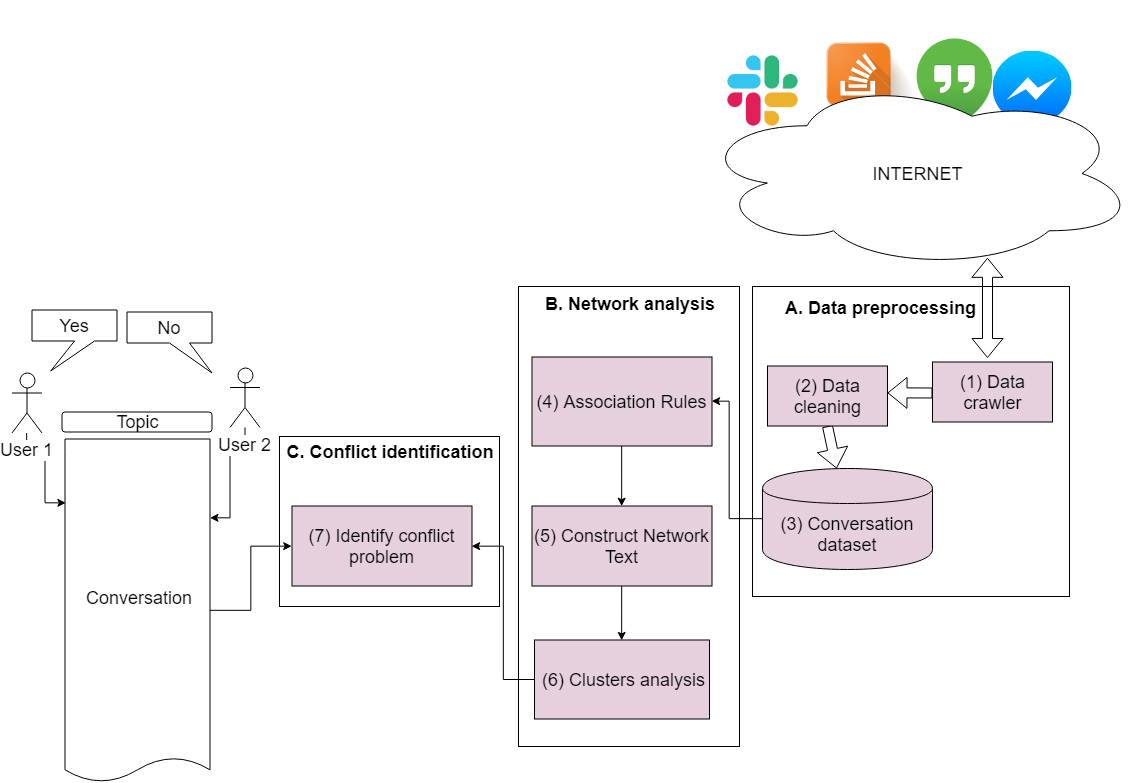
\includegraphics[width=80mm]{32.png}
\end{center}

\end{frame}
\begin{frame}
\frametitle{Objective 2 | Methodology | Data preprocessing}



\begin{columns}
	
	\begin{column}{.55\textwidth}
\textbf{	(1) Data crawler}: crawling data from stackoverflow,\\ hangout, messenger, slackwith a given domain (e.g., statistic)\\
\textbf{	(2) Data cleaning}: Clean content: clean unicode, equation over the conversation\\
\textbf{	(3) Conversation dataset}: save the conversation dataset to the tsv file\\
	\end{column}
	\begin{column}{.55\textwidth}
		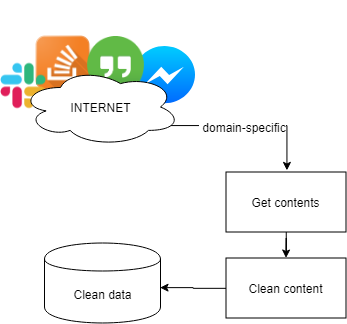
\includegraphics[width=50mm]{dts.png}
	\end{column}
	

\end{columns}
\begin{flushleft}
{\small 	E.g., For slack, hangout, messenger dataset we consider the technical conversation of AI-Educate}\footnote{https://lilabot.com/}
\end{flushleft}

\end{frame}


\begin{frame}
\frametitle{Objective 2 | Methodology}
\textbf{(4) Association rules [*]}: find the interesting association or correlation relationship between dominant words \\


\begin{columns}
	\begin{column}{.55\textwidth}
		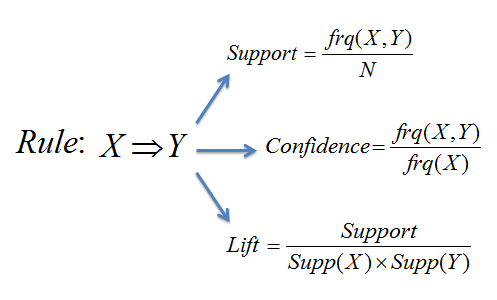
\includegraphics[width=50mm]{AR_1.png}\\
{\tiny 	[*] A. Alamsyah, M. Paryasto, F. J. Putra, R. Himmawan, "Network text analysis to summarize online converstations for marketing intelligence efforts in telecommunication industry", in 2016 ICoICT}
	\end{column}
	\begin{column}{.55\textwidth}
	\begin{itemize}
		\item $Support$: how frequently the itemset appears in the dataset.
		
		
		\item $Confidence$: how often the rule has been found to be true.
		
		
		\item $Lift$: the ratio of the observed support to that expected if X and Y were independent
		
	\end{itemize}
	\end{column}
\end{columns}


\end{frame}


\begin{frame}
\frametitle{Objective 2 | Methodology}
\begin{columns}
	\begin{column}{.35\textwidth}
		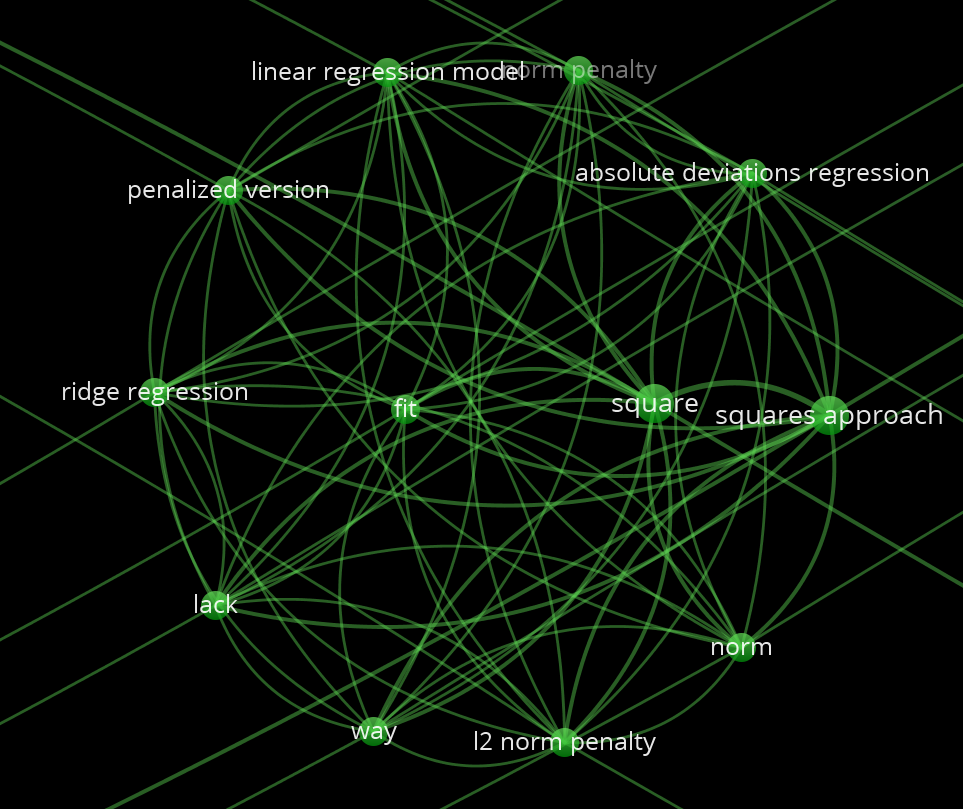
\includegraphics[width=40mm]{nw.png}\\
{\scriptsize 	\textbf{An example of text network}}
	\end{column}

	\begin{column}{.60\textwidth}
(\textbf{5) Construct network text of dominant word}: include weighted edge result for association rule processes\\
\textbf{(6) Network analysis:} create context, keyword, and sense from network text\\
$\rightarrow$ employ centrality to find the most influential words in the networks and modularity to find words cluster/ groups in the network \\
\textbf{(7) Identify conflict problem:} get the conflict problem related to the topic by mapping conversation to clusters analysis\\
	\end{column}
\end{columns}
\end{frame}
\begin{comment}
\begin{frame}
\frametitle{Objective 2 $|$ (A) Definitions extractor}

\begin{itemize}
	\item Extract the definition of  concept from the open source meta-data (e.g., wikipedia, reddit) 
	\item Scrape the definitions of concept from some domain--specific glossary webpage (Breadth First Search) \footnote{https://www.geeksforgeeks.org}
	\item Generate the definition of concept from the other sources which cite this one as a reference
	\item Make the scoring model to evaluate the kind of definitions, SVM is utilized to classify the descriptions
	
\end{itemize}


\end{frame}
\begin{frame}
\frametitle{Objective 2 $|$ (B) Hints generator}
\begin{itemize}
	\item Get the keyword and description from definition extractor
		\item Classify the type of hints based on types of questions (definition, explanation,  definition+explanation, 2 (or more) definitions contrasting each other, list of properties.) by using SVM
			\item Create the auxiliary questions by considering the  keywords in the users' question 
				\item The strategy for now will rely on the comparison of the reference solutions to the question and detection of the bits of the reference solution that can be presented to the users with the template “Think (about) X” / “Consider X” / “Note that X”
\end{itemize}



\end{frame}

\begin{frame}
\frametitle{Objective 2 $|$ (C) Questions and Answers generator}

\begin{itemize}
	\item Each triple consists of a subject, a predicate, and an object. Subjects and objects represent the definition of a concept based on the keywords
	\item Extract the relationship holding between subject and object
	\item Parse data to the types of question to generate the questions
	\item The answer is then generated by taking as input the generated question, the sentence or paragraph used for generating the question, other relevant unstructured data and possibly the user’s answer based on Euclidean distance.
\end{itemize}



\end{frame}

\begin{frame}
\frametitle{Objective 2 $|$ (D) Evaluation of the score of reference}

\par (1) We believe that BLEU
are reasonable evaluation metric: The BLEU [9] metric ranges from 0 to 1. Few translations will attain a score of 1 unless they are identical to a reference translation
\par (2) We use the users experiment testing to evaluate the output




\begin{flushleft}
	{\tiny [9] K. Papineni, S. Roukos, T. Ward, and W.-J. Zhu, "BLEU: A method for automatic evaluation of machine translation, in Proceedings of the 40th Annual Meeting of the Asoociation for Computational Linguistics (ACL), Philadelphia, July 2002, pp. 311--318}
\end{flushleft}
\end{frame}
\begin{frame}
\par 	\textcolor{gray}{(1)  Generate hints to help users solve the topic or problem automatically}
\par \textcolor{gray} {Identify the debated or clarify the problem }
\par (3) \textbf{ Intervene in the conversation to clarify the problem: identify the opportunities for intervention, answer the related topic question of users }
\end{frame}
\begin{comment}
\begin{frame}
\frametitle{Objective 2}

\begin{columns}[T]
	\begin{column}{.5\textwidth}
		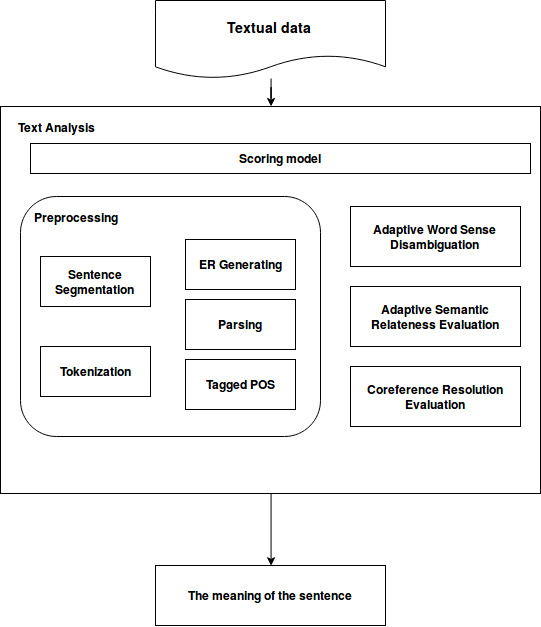
\includegraphics[width=55mm]{f21.jpg}
	\end{column}
	\begin{column}{.5\textwidth}
		
		\begin{itemize}
			\item Step 1: Get the raw text data from the user conversation
			\item Step 2: Process text go extract and compute the score of features 
			\item Step 3: Adapt word sense disambiguation
			\item Step 4: Evalue the semantic relateness and coreference resolution
			\item Step 5: Get the meaning of the sentence
		\end{itemize}
		
	\end{column}
\end{columns}
\end{frame}

\begin{frame}
\frametitle{Process of creating model}
\begin{figure}
	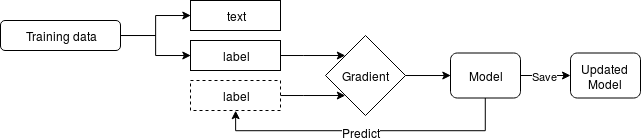
\includegraphics[width=.8\linewidth]{Spacy.png}
\end{figure}

\begin{itemize}
	\item  Our models are \textbf{statistical} and every "decision" are made by \textbf{prediction}
	\item This precision is based on the examples the model has seen during training
	\item We give the model feedback on its prediction in the form of an \textbf{error gradient} of the\textbf{ loss function} that calculates the difference between the training example and the expected output
\end{itemize}
\end{frame}


\begin{frame}
\frametitle{Techniques}
\textbf{Scoring model for definitions (Preprocessing)} 
\begin{columns}[T]
	\begin{column}{.5\textwidth}
		\begin{figure}

				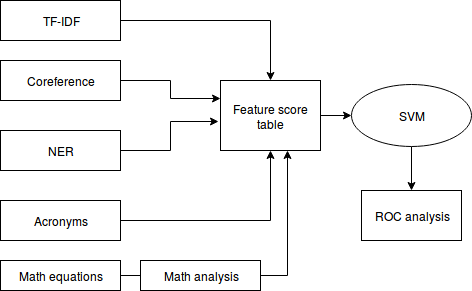
\includegraphics[width=50mm]{u3.png}
		
				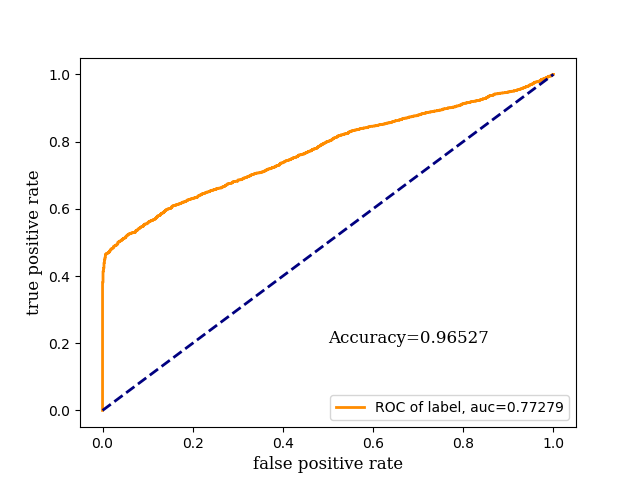
\includegraphics[width=30mm]{testplot.png}

		\end{figure}
	\end{column}
\begin{column}{.5\textwidth}
	\begin{itemize}
		\item Create the features for the scoring model
		\item Compute the score for these ones
		\item Using the SVM algorithm to classify the kind of concept descriptions
		
	\end{itemize}
$\leftarrow$ E.g., extract definitions from wikipedia
\end{column}

\end{columns}


\end{frame}

\begin{frame}
\frametitle{Techniques}
\textbf{Features preprocessing} 
\begin{columns}[T]
	\begin{column}{.5\textwidth}
		
		\begin{itemize}
			\item Recognize the subject, verb, object in a given sentence
			\item Recoginze noun, adj, adv, preposition of a sentence
			\item Recognize the entities in a sentence
			\item Recognize the coreference of a sentence
		\end{itemize}
	\end{column}
	\begin{column}{.6\textwidth}
		
		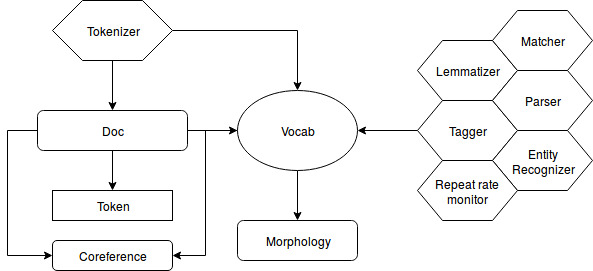
\includegraphics[width=65mm]{f5.jpg}
		
		
	\end{column}
\end{columns}



\begin{flushleft}
	$\rightarrow$ \textit{create the table of features }
\end{flushleft}

\end{frame}

\begin{frame}
\frametitle{Dataset}
\begin{center}
	\textbf{Crawl dataset}\\
	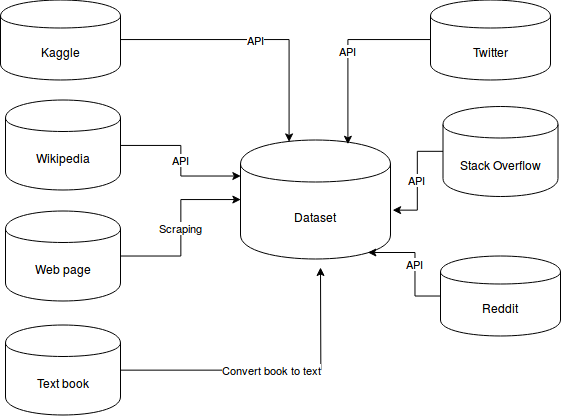
\includegraphics[width=80mm]{dataset.png}
\end{center}
\end{frame}


\begin{frame}
\frametitle{Methodology}
\textbf{Objective 2: Proper intervention}\\

\begin{center}

	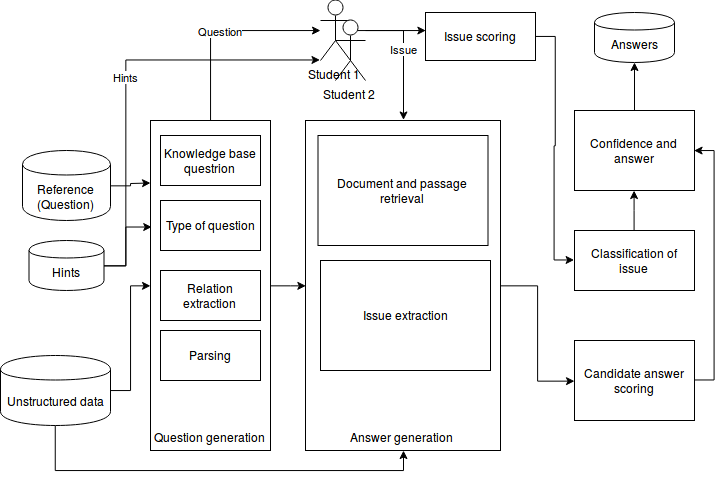
\includegraphics[width=80mm]{interact5.png}
	
\end{center}
\end{frame}
\end{comment}
%keep the title consistence for every section
%put everything label to the block on the diagram
%general diagram
%come to see what is going on in the forum to extract the pattern
%using expert to create the table of evaluation (small training dataset) for opportunies
% what the computer rejected
%____ generating -> give it to the user try to use, and get feedback

%BLUE,  to evaluate the quality of output
%semi-automatic

%what is helpful (say yes or not)
%the professor test first, (OB1: use the data professor interact with student --> converstation -> what kind of intevention....)

\begin{frame}
\par 	\textcolor{gray}{(1)  Generate hints to help users solve the topic or problem automatically}
\par \textcolor{gray}{(2) Identify the debated  problem }
\par (3) \textbf{ Intervene in the conversation to clarify the problem }
\end{frame}
\begin{frame}
\frametitle{Objective 3| Structure}


\begin{figure}
	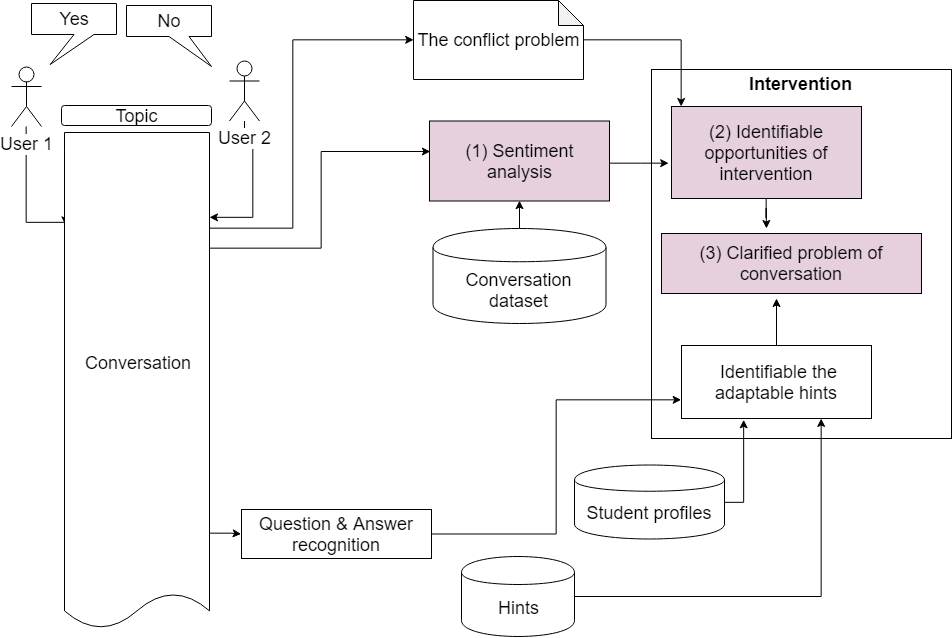
\includegraphics[width=75mm]{58.png}	
	
	
	

\end{figure}

\end{frame}
\begin{frame}
\frametitle{Objective 3 | Methodology | Sentiment analysis}
\begin{columns}
	
	\begin{column}{.5\textwidth}
\begin{figure}
	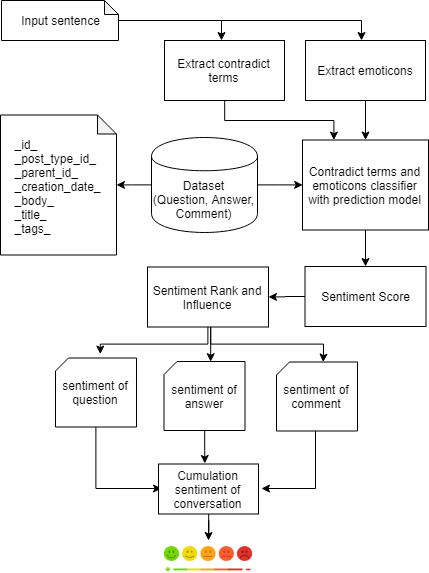
\includegraphics[width=48mm]{st5.png}	
	
\end{figure}
\end{column}
\begin{column}{.5\textwidth}
\begin{itemize}
	\item Listening the conversation
	\item Using SVM in classifying the Emoticons of content
	\item Cummulate the setiment of question, answer, and comment for evaluating the sentiment of conversation
\end{itemize}
{\tiny Ref: L. Ling, S. Larsen, "Sentiment Analysis on Stack Overflow with
Respect to Document Type and
Programming Language", KTH ROYAL INSTITUTE OF TECHNOLOGY}

\end{column}

\end{columns}	
\end{frame}


\begin{frame}
\frametitle{Objective 3 | Methodology | Intervention}
\begin{columns}
	
	\begin{column}{.45\textwidth}
		(2) Identifiable opportunities of intervention: analysis the serious of conversation and conflict problem \\
		
		
		(3) Clarified problem of conversation: give the right intervention\\
	
	\end{column}
	\begin{column}{.55\textwidth}
		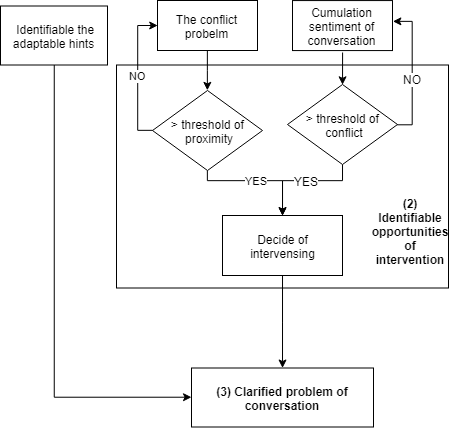
\includegraphics[width=50mm]{tsv3.png}	
	\end{column}
	
\end{columns}
\end{frame}

\begin{frame}
\frametitle{Evaluation measurement}
Because this is the conversation between Human and machine, so we prefer to use the users' experiment test to get feedback score in range (1,5) and expert recommendations.


\end{frame}

\begin{frame}
\frametitle{Evaluation | Approach }


\begin{columns}[onlytextwidth]
	\begin{column}{.45\textwidth}
		\begin{figure}
			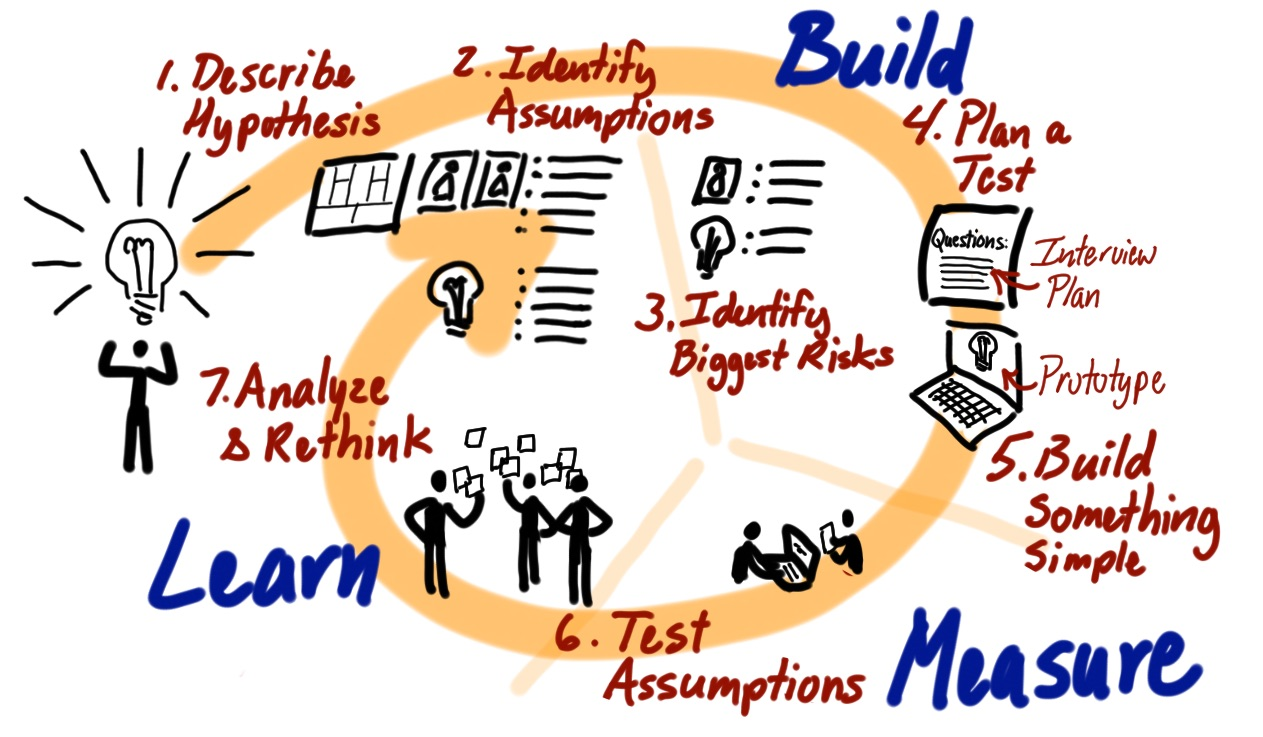
\includegraphics[width=\textwidth]{lsm}
		\end{figure}
		{\tiny 	Source: https://www.jpattonassociates.com/}
	\end{column}
	\hfill
	\begin{column}{.45\textwidth}
		\begin{figure}
			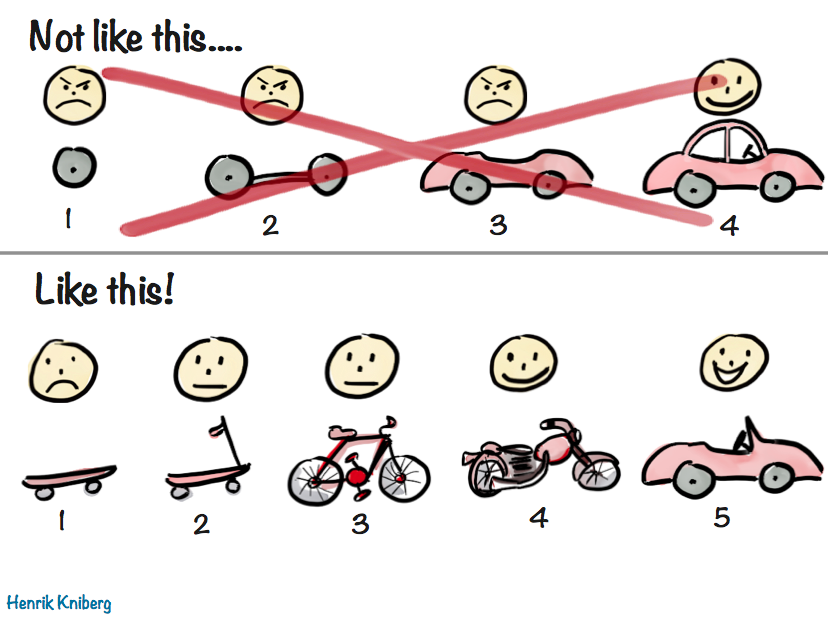
\includegraphics[width=.8\textwidth]{mvp}
		\end{figure}
		{\tiny 	Source: https://quickleft.com}
	\end{column}
\end{columns}

{\scriptsize  $\rightarrow$  We evaluate our system by using the user experiments testing. 
	\begin{itemize}
		\item students' experiments
		\item professor recommendations
	\end{itemize}
	$\rightarrow$ Users: students at the class offline, students on LILA$^4$, friends (if REB is valid) or Amazon Mechanical Turk$^5$}

\begin{flushleft}
	
	{\tiny 4.https://lilabot.com             }
	{\tiny 	 5.https://www.mturk.com/}
\end{flushleft}

\end{frame}

\begin{frame}
\frametitle{Evaluation | Environment}
\begin{figure}
	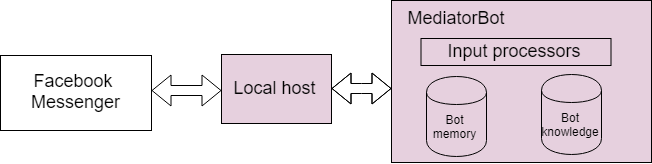
\includegraphics[width=.8\textwidth]{ue1.png}
\end{figure}
\begin{itemize}
	\item {\scriptsize (1) Use the Facebook messenger API to set up the conversation environment}
	\item {\scriptsize (2) Set up the flask server for local host }
	\item {\scriptsize (3) Process the conversation with the given bot memory and knowledge }
	\item {\scriptsize (4) Make the report feedback statistic evaluation (\url{https://docs.gogle.com/forms/u/0/ })}
	\item {\scriptsize (5) Using Cohen's kappa for evaluating the agreement of human and machine experiment }
\end{itemize}


\end{frame}


\begin{frame}
\frametitle{Achievements}
(1) 3 years Mitacs accelerate grant for Natural Language Generation for Intelligent Tutoring Systems \\
\begin{center}
	
\end{center}
(2) Directly apply the results to LILA and Korbit systems at Ai-educate Inc \\

\url{https://lilabot.com/} \\

\begin{center}
	
\end{center}
(3) Get the good feedback from the students though LILA system (Ai-educate has the REB for this experiement)



\end{frame}
\begin{frame}
\frametitle{Achievements}
+ Experiment setup: graduate and undergraduate students from McGill COMP-551 from 6/2/2019 - 8/2/2019

{\scriptsize \begin{table}[]
	\begin{tabular}{|l|l|l|}
		\hline
		& \begin{tabular}[c]{@{}l@{}}Human-Generated\\  Hints\end{tabular} & \begin{tabular}[c]{@{}l@{}}Machine-Generated \\ Hints\end{tabular} \\ \hline
		Sessions (Users)                                                                                                                                                    & {\color[HTML]{333333} 36}                                        & {\color[HTML]{333333} 36}                                          \\ \hline
		\begin{tabular}[c]{@{}l@{}}Number of times text-based hint \\ was shown (including the times it\\  was shown after the user clicked \\ “I don’t know”)\end{tabular} & 30 (100\%)                                                       & 19 (100\%)                                                         \\ \hline
		\begin{tabular}[c]{@{}l@{}}Number of times users improved \\ their next solution attempt after \\ hint was shown\end{tabular}                                       & 8 (26.67\%)                                                      & \textbf{8 (42.11\%)                                                      }  \\ \hline
		\begin{tabular}[c]{@{}l@{}}Number of times users gave a \\ “CORRECT” next solution attempt \\ after hint was shown\end{tabular}                                     & 5 (16.67\%)                                                      & \textbf{6 (31.58\%)                                                        }\\ \hline
	\end{tabular}
\end{table}}
\textit{Source: Ai-educate}
\end{frame}

\begin{comment}
\subsection{} % A subsection can be created just before a set of slides with a common theme to further break down your presentation into chunks

\begin{frame}
\frametitle{Introduction}
\begin{columns}[T]
	
\begin{column}{.45\textwidth}
	\begin{figure}
		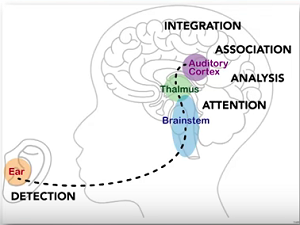
\includegraphics[width=50mm]{sound_processing_courtesy_asha.png}
		https://www.autismspeaks.org
	\end{figure}
\end{column}

\begin{column}{.6\textwidth}
	\begin{itemize}
		\item Auditory processing is defined as what we do with what we hear \footnote{Katz  \&  Tillery,  2004}
		\item Auditory Processing Disorder (APD) is a condition where someone has normal hearing, but the auditory system does not faithfully bring information to the brain \footnote{https://www.sac-oac.ca}
		\item \textbf{Approximate 2-4\% of school age children have APD} \footnote{http://www.ementalhealth.ca/}
		\item Autism and auditory processing disorders often overlap\footnote{https://www.autismspeaks.org}
	\end{itemize}
\end{column}
\end{columns}


\end{frame}
\begin{frame}
\frametitle{Challenging}
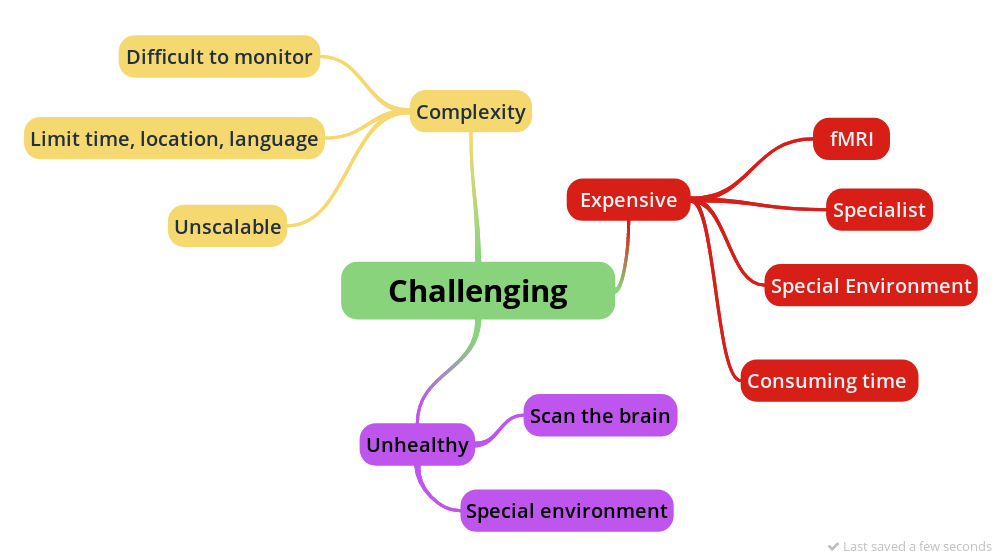
\includegraphics[width=120mm]{mind.jpg}

\end{frame}
\begin{frame}
\frametitle{Objectives}
Propose an AI model (virtual assitance) named \textcolor{blue}{\textbf{MedicBot}} to assit in diagnosing, monitoring, and training of the children with APD problem with low price, healthy, and convinent
\begin{columns}
	\begin{column}{.3\textwidth}
\begin{center}
		
\includegraphics[width=30mm]{MedicBot.png}
	
\textbf{	MedicBot}
\end{center}

	\end{column}
\begin{column}{.7\textwidth}


\begin{itemize}
	\item Diagnose APD symptoms based on \textcolor{blue}{conversation} with the considered children
	\item Create a Training Therapy Model Assitance (adaptable)
	\item Build the Reinforcement Learining (RL) Model to monitor the progress of APD treatment
\end{itemize}



\end{column}
\end{columns}
\end{frame}

\section{Problem statement}
\section{Literature survey}
\section{Motivations}
\section{Objectives}
%------------------------------------------------
\section{Methodology } % Sections can be created in order to organize your presentation into discrete blocks, all sections and subsections are automatically printed in the table of contents as an overview of the talk
%------------------------------------------------
\subsection{} % A subsection can be created just before a set of slides with a common theme to further break down your presentation into chunks

\begin{frame}
	\frametitle{Methodology}
	\begin{itemize}
		\item Analysis  the  given  APD  symptoms  by  speech  	
		recognition  based  on  Deep  learning
		
		\item \color{gray} Analysis  the  given  APD  therapy  and  recommend  the
		
		treatment  to  the  APD  children.  Apply  a  natural  language
		
		processing  (NLP)  to  generate  sentences  and  exploit  Deep
		
		learning  to  understand  the  context  of  the  speech
		
		\item Monitoring  the  process  of  APD  treatment  by  using  speech  analysis  based  on  Deep
		
		learning
	\end{itemize}

\end{frame}


%------------------------------------------------

%------------------------------------------------
\begin{frame}
\frametitle{Implementation}
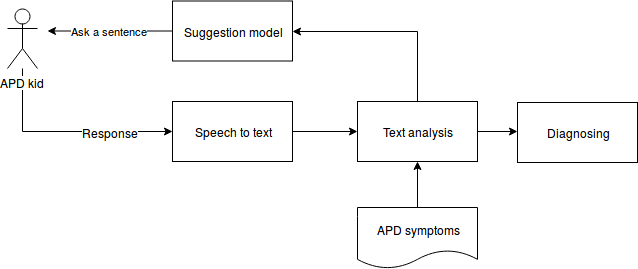
\includegraphics[width=120mm]{process.png}
\end{frame}

\begin{frame}
\frametitle{Techniques}
\textbf{Convert speech to text}
\begin{columns}[T]
		\begin{column}{.5\textwidth}
		
		\begin{itemize}
			
		\item	\textbf{Acoustic modeling} represents the relationship between linguistic units of speech and audio signals.
		\item	\textbf{Language modeling} matches sounds with word sequences to help distinguish between words that sound similar.
			
		\end{itemize}
		
	\end{column}
	\begin{column}{.5\textwidth}
				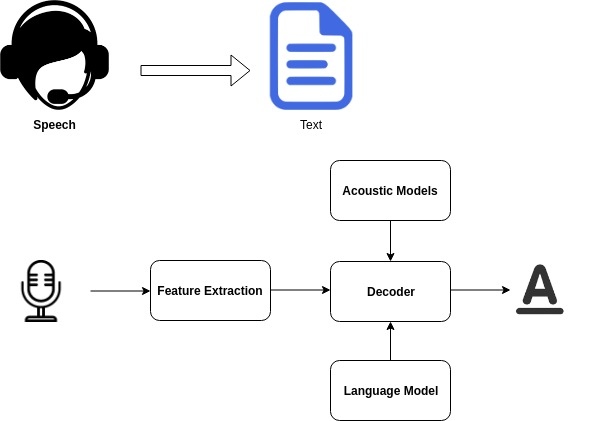
\includegraphics[width=65mm]{f1.jpg}
	\end{column}

\end{columns}
 {\small We evaluated the quality of output by using two factors:\footnote{https://pypi.org/project/SpeechRecognition/}\\

\textbf{Accuracy} and \textbf{Speed} }

\end{frame}

%------------------------------------------------


\begin{frame}
\frametitle{Techniques}
\textbf{Proposal for the objective 1 solution}
\begin{columns}[T]
	\begin{column}{.5\textwidth}
		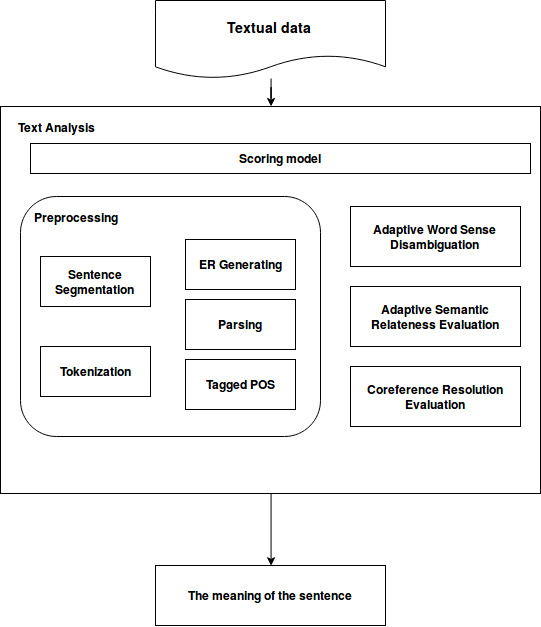
\includegraphics[width=55mm]{f21.jpg}
	\end{column}
	\begin{column}{.5\textwidth}
		
		\begin{itemize}
			\item Step 1: Get the raw text data from the user conversation
			\item Step 2: Process text go extract and compute the score of features 
			\item Step 3: Adapt word sense disambiguation
			\item Step 4: Evalue the semantic relateness and coreference resolution
			\item Step 5: Get the meaning of the sentence
		\end{itemize}
		
	\end{column}
\end{columns}

\end{frame}
\begin{frame}
\frametitle{Dataset}
\textbf{Open Dataset}
\begin{itemize}
{\scriptsize   	\item (NLVR) A Corpus of Natural Language for Visual Reasoning, 2017
	\item (MS MARCO) MS MARCO: A Human Generated MAchine Reading COmprehension Dataset, 2016
	\item (NewsQA) NewsQA: A Machine Comprehension Dataset, 2016 
	\item (SQuAD) SQuAD: 100,000+ Questions for Machine Comprehension of Text, 2016
\item 	(GraphQuestions) On Generating Characteristic-rich Question Sets for QA Evaluation, 2016 
\item 	(Story Cloze) A Corpus and Cloze Evaluation for Deeper Understanding of Commonsense Stories, 2016 
\item 	(Children's Book Test) The Goldilocks Principle: Reading Children's Books with Explicit Memory Representations, 2015 
\item 	(SimpleQuestions) Large-scale Simple Question Answering with Memory Networks, 2015
\item 	(WikiQA) WikiQA: A Challenge Dataset for Open-Domain Question Answering, 2015
\item 	(CNN-DailyMail) Teaching Machines to Read and Comprehend, 2015 
\item 	(QuizBowl) A Neural Network for Factoid Question Answering over Paragraphs, 2014 
\item 	(MCTest) MCTest: A Challenge Dataset for the \item Open-Domain Machine Comprehension of Text, 2013 
\item (QASent) What is the Jeopardy model? A quasisynchronous grammar for QA, 2007 }
\end{itemize}


\end{frame}
\begin{frame}
\frametitle{Dataset}
\begin{center}
	\textbf{Crawl dataset}\\
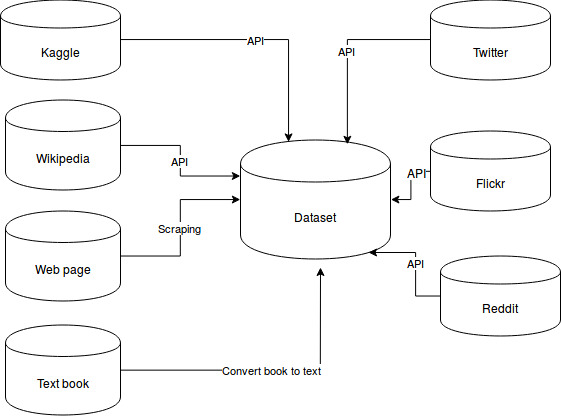
\includegraphics[width=80mm]{f9.jpg}
\end{center}
\end{frame}

\begin{frame}
\frametitle{Dataset}
\textbf{Paraphase database (PPDB)}
\begin{itemize}
	\item \textbf{PPDB}\footnote{http://paraphrase.org} is an automatically extracted database containing millions paraphrases in 16 different languages. 
	\item 
	The goal of PPBD is to improve language processing by making systems more robust to language variability and unseen words. 
	\item The entire PPDB resource is freely available under the Creative Commons Attribution 3.0 United States License.
	\item PPDB contains over 150 million paraphrase rules covering three paraphrase types lexical (single word), phrasal (multiword), and syntactic restructuring rules
\end{itemize}




\end{frame}


\begin{frame}
\frametitle{Chatbot}
\begin{columns}[T]
	\begin{column}{.5\textwidth}
		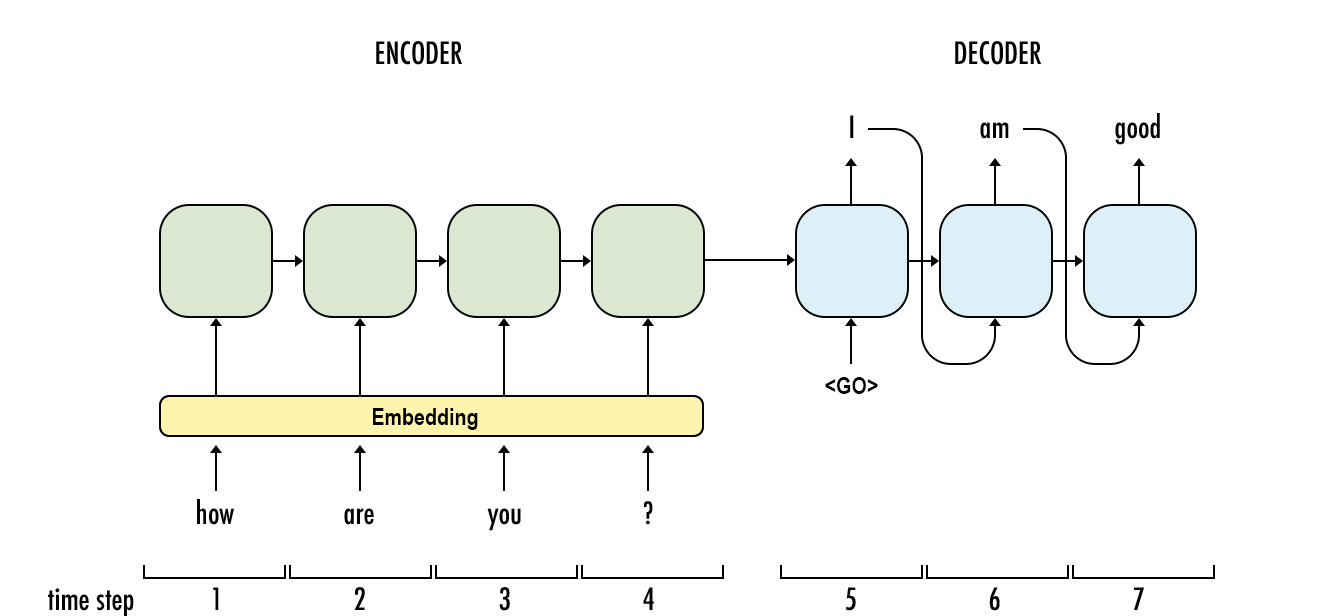
\includegraphics[width=65mm]{seq2seq.png}
		\begin{itemize}
		{\scriptsize 	\item $<PAD>$: During training, inputs in these batches all need to be the same width for the network to do its calculation. 
			\item $<EOS>$: It allows us to tell the decoder where a sentence ends, and it allows the decoder to indicate the same thing in its outputs as well.
		}
		\end{itemize}
	\end{column}
	\begin{column}{.5\textwidth}
		
		\begin{itemize}
{\scriptsize 
			\item $<UNK>$: If you’re training your model on real data, you’ll find you can vastly improve the resource efficiency of your model by ignoring words that don’t show up often enough in your vocabulary to warrant consideration. We replace those with $<UNK>$.
	
		\item $<GO>$: This is the input to the first time step of the decoder to let the decoder know when to start generating output.}
		\end{itemize}
		
	\end{column}
\end{columns}

\end{frame}


\begin{frame}
\frametitle{APD Symptoms}
\begin{table}[]
	\begin{tabular}{|l|llll}
		\cline{1-1}
		\textbf{Listening} &  &  &  &  \\ \cline{1-1}
	Has difficulty locating a sound source.	&  &  &  &  \\ \cline{1-1}
	Has difficulty hearing in noisy background. 	&  &  &  &  \\ \cline{1-1}
	Often asks for repetition or clarification 	&  &  &  &  \\ \cline{1-1}
	\textbf{Speaking}	&  &  &  &  \\ \cline{1-1}
Has difficulty answering open--ended questions	&  &  &  &  \\ \cline{1-1}
May speak in oversimplified short sentences with difficulties in syntax  	&  &  &  &  \\ \cline{1-1}
Mispronounced words, especially long words. 	&  &  &  &  \\ \cline{1-1}
\textbf{Phonological Awareness}	&  &  &  &  \\ \cline{1-1}
Has difficulty focusing during conversations	&  &  &  &  \\ \cline{1-1}
Forgets information that is easily heard 	&  &  &  &  \\ \cline{1-1}
	\end{tabular}
	\caption{A part of checklist for assessing whether the child with APD\footnote{https://kidshear.com.au}}
	\label{1}
\end{table}

\end{frame}

\begin{frame}
\frametitle{Process of creating model}
\begin{figure}
		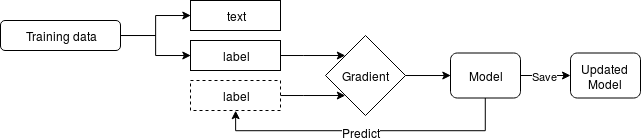
\includegraphics[width=.8\linewidth]{Spacy.png}
\end{figure}

\begin{itemize}
	\item  MedicBot's models are \textbf{statistical} and every "decision" she makes is a \textbf{prediction}
	\item This precision is based on the examples the model has seen during training
	\item We give the model feedback on its prediction in the form of an \textbf{error gradient} of the\textbf{ loss function} that calculates the difference between the training example and the expected output
\end{itemize}
\end{frame}


\begin{frame}
\frametitle{Techniques}
\textbf{Scoring model} 
\begin{columns}[T]
		\begin{column}{.5\textwidth}
			\begin{itemize}
				\item Create the features for the scoring model
				\item Compute the score for these ones
				\item Using the K-Mean Clustering algorithm to cluter the kid
				\item Apply the Elbow and K-validation algorithm to optimize the K-value of K-Mean Clustering algorithm
				\item Make the score table of considered kids
			\end{itemize}
		\end{column}
		\begin{column}{.7\textwidth}
			
			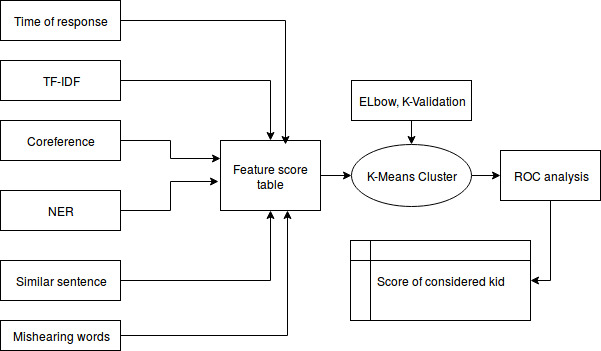
\includegraphics[width=65mm]{f6.jpg}
			
		\end{column}
	\end{columns}
	
\end{frame}

\begin{frame}
\frametitle{Techniques}
\textbf{Preprocessing} 
\begin{columns}[T]
	\begin{column}{.5\textwidth}
		\begin{itemize}
			\item Recognize the subject, verb, object in a given sentence
			\item Recoginze noun, adj, adv, preposition of a sentence
			\item Recognize the entities in a sentence
			\item Recognize the coreference of a sentence
		\end{itemize}
	\end{column}
	\begin{column}{.6\textwidth}
		
		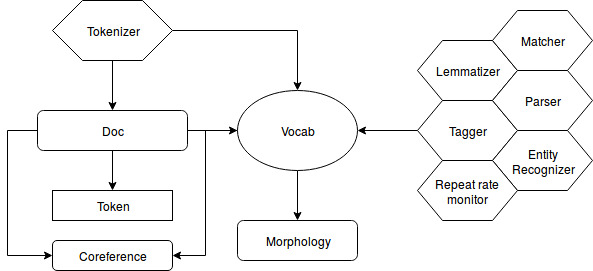
\includegraphics[width=65mm]{f5.jpg}
		
		
	\end{column}
\end{columns}



\begin{flushleft}
	$\rightarrow$ \textit{create the table of features }
\end{flushleft}

\end{frame}
\begin{frame}

\begin{table}[]
	\begin{tabular}{lllll}
		\cline{1-2}
		\multicolumn{1}{|l|}{time of response } & \multicolumn{1}{l|}{$\sum_{t=0}^{T}(t_i)$, $t_i$ the duration of one sentence} &  &   &  \\ \cline{1-2}
		\multicolumn{1}{|l|}{tf-idf(k,d,D)} & \multicolumn{1}{l|}{\begin{tabular}[c]{@{}l@{}}$tf(k,d)\times idf(k,D)$, $k$: term $k$\\ $d$: document $d$; and $d \in D$ \end{tabular} } &  &  &  \\ \cline{1-2}
		\multicolumn{1}{|l|}{coreference} & \multicolumn{1}{l|}{coreference resolution evaluation} &  &  &  \\ \cline{1-2}
		\multicolumn{1}{|l|}{ner} & \multicolumn{1}{l|}{name entity recognization}                                              &  &  &  \\ \cline{1-2}
			\multicolumn{1}{|l|}{similar sentence} & \multicolumn{1}{l|}{similarity evaluation}                                              &  &  &  \\ \cline{1-2}
				\multicolumn{1}{|l|}{mishearing word} & \multicolumn{1}{l|}{spelling and  grammar checking evaluation}                                              &  &  &  \\ \cline{1-2}
					\multicolumn{1}{|l|}{elbow algorithm} & \multicolumn{1}{l|}{choose a small value of k that still has a low SSE}                                              &  &  &  \\ \cline{1-2}
			\multicolumn{1}{|l|}{ROC analysis} & \multicolumn{1}{l|}{		 Receiver Operating Characteristic analysis}                                              &  &  &  \\ \cline{1-2}

	\end{tabular}
\end{table}


\end{frame}
\begin{frame}
\frametitle{Implementation}

\begin{table}[]
	\begin{tabular}{|l|l|}
		\hline
		\textbf{}                                           Requirements              & Content                                   \\ \hline
		\textbf{Python}                                                         & \begin{tabular}[c]{@{}l@{}} 2.6, 2.7, or 3.3+ \end{tabular} \\ \hline
		\textbf{PocketSphinx}                                              & \begin{tabular}[c]{@{}l@{}} large vocabulary speaker independent \\recognition system\end{tabular} \\ \hline
		\begin{tabular}[c]{@{}l@{}}\textbf{PyAudio}\end{tabular} & \begin{tabular}[c]{@{}l@{}} 0.2.11+ (required only if you need to\\ use microphone input, Microphone)\end{tabular} \\ \hline
		
		\textbf{SpeechRecognition}                                                         & \begin{tabular}[c]{@{}l@{}} a process in which a computer or device record\\ the speech of humans and convert it into text  \end{tabular} \\ \hline
		\textbf{Google API Client}                                                         & \begin{tabular}[c]{@{}l@{}} use the Google Cloud Speech API \end{tabular} \\ \hline
		\textbf{FLAC encoder}                                                         & \begin{tabular}[c]{@{}l@{}}if the system is not x86-based \\Windows/Linux/OS X \end{tabular} \\ \hline
	\end{tabular}
	\caption{Requirements of environment}
	\label{tab:setup}
\end{table}
\end{frame}
\begin{frame}
\frametitle{Implementation}
\begin{table}[]
	\begin{tabular}{|l|l|}
		\hline
		\textbf{}                                           Requirements              & Content                                   \\ \hline
		\textbf{SpaCy}                                                         & \begin{tabular}[c]{@{}l@{}} Industrial-Strength NLP \end{tabular} \\ \hline
		\textbf{NeuralCoref}                                              & \begin{tabular}[c]{@{}l@{}} Coreference Resolution in spaCy with Neural Netwo-\\rks \end{tabular} \\ \hline
		\begin{tabular}[c]{@{}l@{}}\textbf{NLTK}\end{tabular} &  \begin{tabular}[c]{@{}l@{}}Natural Language toolkit\end{tabular} \\ \hline
		
		\begin{tabular}[c]{@{}l@{}}\textbf{Scikit-learn} \\\textbf{Tensorflow} \\\textbf{Pytorch}   \end{tabular}                                                     & \begin{tabular}[c]{@{}l@{}} Machine learning library  \end{tabular} \\ \hline
		\textbf{ELMo}                                                         & \begin{tabular}[c]{@{}l@{}} Embeddings from Language Models \end{tabular} \\ \hline
	
	\end{tabular}
	\caption{Requirements of environment}
	\label{tab:setup}
\end{table}
\end{frame}
%\begin{frame}
%\frametitle{Coreference resolution evaluation}
%\begin{figure}
%	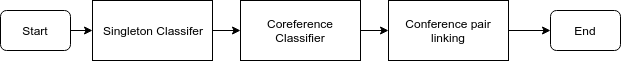
\includegraphics[width=.9\linewidth]{Coreference.png}
%\end{figure}
%\begin{itemize}
%	\item \textbf{Singleton classifier}: This classifier 
%	considers  five  representations  which  are  word,  dependency,  
%	string,  numeric,  and  mention
%	\item \textbf{Coreference classifier}: This   
%	classifier     considers     six     representations,     which     are     
%	dependency,  antecedent,  mention,  pair  string,  pair  numeric,  
%	and  mention  pair.
%	\item \textbf{Coreference pair linking} - Mention Ranking Model: The coreference classifier has predicted coreferent scores 
%	for  all  mention  pairs  of  a  targeted  mention
%\end{itemize}
%\end{frame}



\begin{frame}

\frametitle{Unit tests of the system}

\begin{figure}
	
		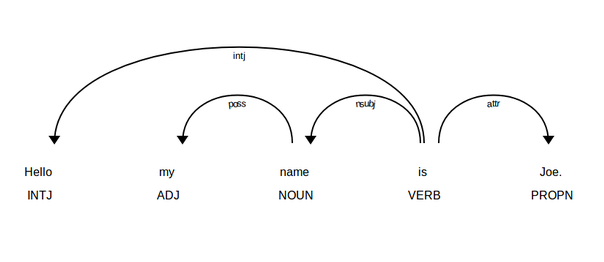
\includegraphics[width=.7\linewidth]{01.png}
		\includegraphics[width=.9\linewidth]{02.png}
		\includegraphics[width=.7\linewidth]{03.png}
	

\end{figure}

\end{frame}
%------------------------------------------------
\begin{frame}
\frametitle{Methodology}
\begin{itemize}
	\item \textcolor{gray}{Analysis  the  given  APD  symptoms  by  speech  
		recognition  based  on  Deep  learning}
	\item Analysis  the  given  APD  therapy  and  recommend  the
	
	treatment  to  the  APD  children.  Apply  a  natural  language
	
	processing  (NLP)  to  generate  sentences  and  exploit  Deep
	
	learning  to  understand  the  context  of  the  speech
	
	\item \textcolor{gray} {Monitoring  the  process  of  APD  treatment  by  using  speech 	 analysis  based  on  Deep learning}
	
\end{itemize}

\end{frame}

\begin{frame}
\frametitle{Techniques}
\textbf{Proposal for the objective 2 solution}
\begin{columns}	
\begin{column}{.5\textwidth}
	\includegraphics[width=65mm]{f3(1).jpg}
\end{column}
\begin{column}{.5\textwidth}
	
	\begin{itemize}
		\item Propose a training therapy to the APD kid based on the diagnosing report and Task recommendation model
		\item Monnitor the progress of therapy
		\item Update the monitoring data
		\item Suggest the fit training therapy by using reinforcement learning based on recommendation system
	\end{itemize}
	
\end{column}
\end{columns}
\end{frame}


\begin{frame}
\textbf{Task recommendation model \footnote{https://www.thebsa.org.uk}}
\begin{center}
	\includegraphics[width=100mm]{11.png}
\end{center}
\end{frame}

\begin{frame}
\textbf{Tasks and criteria}\\
\begin{columns}	
	\begin{column}{.5\textwidth}
		\includegraphics[width=65mm]{RL.jpg}
	\end{column}
	\begin{column}{.5\textwidth}
	\begin{itemize}
		\item State space $\mathcal{S}$: A state $s_t = \{s_t^i\}, i = (1,N)$
		\item  Action space $\mathcal{A}$: An action $a_t = \{a_t^j\}, j =( 1, K)$
		\item Reward $\mathcal{R}$: $r(s_t,a_t)$ according to the user's feedback
		\item Transition probability $\mathcal{P}$: $p(s_{t+1}|s_t,a_t)$ defines the probebility of state transition from $s_t$ to $s_{t+1}$ when Recommender Agent takes action $a_t$
	\end{itemize}
\end{column}
\end{columns}
\end{frame}



%------------------------------------------------
\begin{frame}
\frametitle{Methodology}
\begin{itemize}
\item \textcolor{gray}{Analysis  the  given  APD  symptoms  by  speech  
recognition  based  on  Deep  learning}
\item \textcolor{gray} {Analysis  the  given  APD  therapy  and  recommend  the 	treatment  to  the  APD  children.  Apply  a  natural  language 	processing  (NLP)  to  generate  sentences  and  exploit  Deep 	learning  to  understand  the  context  of  the  speech}

\item Monitoring  the  process  of  APD  treatment  by  using  speech analysis  based  on  Deep learning

\end{itemize}

\end{frame}
%------------------------------------------------


\begin{frame}
\frametitle{Techniques}
\textbf{Proposal for the objective 3 solution}\\


\begin{itemize}
\item Convert the APD speech to text
\item Analysis the meaning of the text
\item Make the score of the benchmark table

\item Make the client-server model to monitor and evaluate the progress of each patient
\end{itemize}


\end{frame}

\begin{frame}
\begin{figure}
\includegraphics[width=65mm]{f4.jpg}
\end{figure}

Describe the score of the training for the respective user at home
\begin{table}[]
	\begin{tabular}{|l|l|l|l|l|}
		\hline
		\textbf{}                                                         & Observation & Assessment & \begin{tabular}[c]{@{}l@{}}Therapy \\ lesson\end{tabular} & Other \\ \hline
		Listening                                                         &             &            &                                                              &       \\ \hline
		Speaking                                                          &             &            &                                                              &       \\ \hline
		\begin{tabular}[c]{@{}l@{}}Phonological \\ Awareness\end{tabular} &             &            &                                                              &       \\ \hline
	\end{tabular}
	\caption{Benchmark table}
	\label{2}
\end{table}
\end{frame}

\begin{frame}
\frametitle{Client and Master MedicBot}
\begin{columns}	
	\begin{column}{.5\textwidth}
		\includegraphics[width=55mm]{client.jpg}
	\end{column}
	\begin{column}{.5\textwidth}
		
			\includegraphics[width=55mm]{Master.jpg}
		
	\end{column}
\end{columns}
MedicBot Client collects data from User and then send them to the MedicBot Master to store and analysis more (if the problem needs specialists)
\end{frame}
\end{comment}
\section{Work plan}

\begin{frame}
\frametitle{Work plan}
\begin{figure}
	\includegraphics[width=100mm]{plan2.png}
	\caption{Work schedule}
\end{figure}

\begin{columns}[T]
	\begin{column}{.7\textwidth}
	\textbf{Journals:}
	\par [1] Journal of Artificial Intelligence Research 
	\par [2] Technology, Knowledge and Learning
	\par [3] Education and Information Technologies
		
	\end{column}
	\begin{column}{.3\textwidth}
	\textbf{Finished courses:}
	\par (1) DGA1005
	\par (2) MTI830

	\end{column}
\end{columns}



\end{frame}




\begin{frame}{}
\centering \Huge
\emph{Thank You}
\end{frame}


\begin{comment}
\begin{frame}
\frametitle{Training spaCy’s Statistical Models}
{\footnotesize \par + spaCy is the best way to prepare text for deep learning. 
 \par + with spaCy, you can easily construct linguistically sophisticated statistical models for a variety of NLP problems
 \par + spaCy's models are statistical and every "decision" they make is a prediction. This prediction is based on the examples the model has seen during training. 
 	\includegraphics[width=100mm]{Spacy.png}}
 {\tiny Reference:}
 {\tiny \href{https://explosion.ai/demos/displacy}{https://explosion.ai/demos/displacy}
 }
\end{frame}

\begin{frame}
\par (1) Syntax tree demo:  \href{https://explosion.ai/demos/displacy}{Syntax tree display}
\par (2) Seq2Seq demo: 
\href{http://jalammar.github.io/visualizing-neural-machine-translation-mechanics-of-seq2seq-models-with-attention/}{Visualizing A Neural Machine Translation Model (Mechanics of Seq2seq Models With Attention)}
\par (3) 
BFS demo: 
\href{https://www.cs.usfca.edu/~galles/visualization/BFS.html}{
	Breadth-First Search
}

\end{frame}
%------------------------------------------------
\end{comment}


\end{document}